\section{Methods}

\subsection{Data}

%B: IMO: The data subsection would be better organized with parts, (1) ploidy, (2) breeding system, (3) tree, (4) models, (5) model selection and statistical inference.
% E: I changed the subsectioning, but to a different arrangement: (1) Data, (2) Models, (3) Statistical inference.  With subsubsections as necessary.

Chromosome number data were obtained for all Solanaceae taxa in the Chromosome Counts Database \citep[CCDB;][]{rice_2015}, and the ca.~14,000 records were curated semi-automatically using the \mbox{CCDBcurator} R package \citep{rivero_2019}.
CCDB contains records from original sources that have multiple complex symbol patterns denoting multivalence, or irregularites of chromosome counts.
After a first round of automatic cleaning, we examined results by hand and corrected records as necessary.
Our hand-curated records were also contrasted against the ploidy dataset from \citet{robertson_2011}, original references therein, and against ploidy data in the C-value DNA dataset from \citet{bennett_2005}.
By comparing three different sources of information, we were able to code taxa as diploid, $D$, or polyploid, $P$.
For the majority of species, ploidy was assigned according to information from the original publications included in the  C-value DNA dataset \citep{bennett_2005}.
For taxa without ploidy information but with information about chromosome number, we assigned ploidy based on the multiplicity of chromosomes within the genus/family, or based on SI/SC classification.
For example, \textit{Solanum betaceum} did not have information about ploidy level but it has 24 chromosomes, so since $x=12$ is the base chromosome number of the genus \textit{Solanum} \citep{olmstead_2007}, we assigned \textit{S.~betaceum} as diploid. 
Additionally, because of the absence of SI polyploids (explained above and below), species known to be SI could be scored as diploid.
Species with more than one ploidy level were assigned the most frequent ploidy level recorded or the smallest ploidy in case of frequency ties.

Breeding system states were scored as self-incompatible, $I$, or self-compatible, $C$, based on results curated from the literature and original experimental crosses \citep[as compiled in][]{igic_2006, goldberg_2010, robertson_2011, goldberg_2012}.
Most species could unambiguously be coded as either $I$ or $C$ \citep{raduski_2012}.
Following previous work, we coded any species with a functional SI system as $I$, even if SC or dioecy was also reported.
Dioecious species without functional SI were coded as $C$.
% E: I am trying to stick with I/C when talking about the state values, but using SI/SC when talking about the meaning of the trait (because this what people use normally). 
%R- Okay- I was getting confused as well thanks for clarifying

Resolution of taxonomic synonymy followed Solanaceae Source \citep{solsource}. 
Hybrids and cultivars were excluded because ploidy and breeding system can be affected by artificial selection during domestication.
Following the reasoning outlined in \citet{robertson_2011}, we closely examined the few species for which the merged ploidy and breeding system data indicated the presence of self-incompatible polyploids.
Although SI populations frequently contain some SC individuals, and diploid populations frequently contain some polyploid individuals, in no case did we find convincing data for a naturally occurring SI polyploid population  \citep[discussed in][]{robertson_2011}.
%B rm: The single instance of an SI polyploid individual appears to be an allopentaploid hybrid of \textit{Solanum oplocense} Hawkes x \textit{Solanum gourlayii} Hawkes, reported by \citet{camadro_1981}.
% Under exceedingly rare circumstances, it is possible for polyploids containing multiple copies of S-loci to remain SI, so long as they express a single allele at the S-locus \citep[discussed in][]{robertson_2011}.
Because of the resulting absence of polyploid SI populations, as well as the functional explanation for polyploidy disabling gametophytic SI systems with non-self recognition (see the Introduction), we consider only three observed character states: self-incompatible diploids $(ID)$, self-compatible diploids $(CD)$, and self-compatible polyploids $(CP)$.

Matching our character state data to the largest time-calibrated phylogeny of Solanaceae \citep{sarkinen_2013} yielded 651 species with ploidy and/or breeding system information on the tree.
% Fixed!
Of these, 368 had information for both states.
The number of species in each combination of states is summarized in \cref{figure:stateclassifications}A.
We retained all 651 species in each of the analyses below because pruning away tips lacking breeding system in the ploidy-only analyses (and vice versa) would discard data that could inform the diversification models.
A total of 372 taxa without any information about breeding system or ploidy were excluded.
%Tips without trait data might not improve point estimation of diversification parameters while increasing uncertainty in the estimates of trait linked diversification
% R-This is very important but I have removed it because I think it is a full on paper by its own
%Including this many more species would have prohibitively slowed our analyses, especially those implementing the most complex models.

The Supplementary Information contains citations for the numerous original data sources. % FIXME (and say here how many refs?) %B: no need for an additional counting and updating headache?
The Dryad archive contains the data and tree files used for analyses. % FIXME
% \url{https://github.com/roszenil/solploidy}  E: we should use dryad instead, because github repos are not guaranteed to last

\subsection{Models}

In order to test our hypotheses about lineage diversification and trait macroevolution, we fit 29 state-dependent speciation and extinction models \citep[BiSSE, MuSSE, HiSSE;][]{maddison_2007, fitzjohn_2012, beaulieu_2016}.
SSE models contain parameters that describe per-lineage rates of speciation and extinction, specific to each character state (denoted $\lambda$ and $\mu$, respectively, with subscripts to indicate the state), along with rates of transitions between states (denoted $\rho$ for polyploidization, $\delta$ for diploidization, and $q_{IC}$ for loss of self-incompatibility).
The full set of models and all their rate parameters are detailed in \cref{fig:allmodels}.
Here, we summarize how each model allows us to assess whether diversification is best explained by variation in ploidy, breeding system, their combination, or some unknown factor.

\subsubsection{Ploidy and diversification}

In order to investigate the association between ploidy level and diversification, we first employed a model (labeled M1), previously used by \citet{mayrose_2011}, with each species classified as diploid $(D)$ or polyploid $(P)$.
Although this model can be powerful in studies of trait evolution, it is prone to incorrectly reporting that a trait is associated with diversification differences \citep{maddison_2015, rabosky_2015}.
We therefore define several models that incorporate additional forms of diversification rate heterogeneity.

The second ploidy model (M2) includes a binary hidden trait that subdivides each observed state.
In this trait-independent model known as CID \citep{beaulieu_2016}, hidden traits can affect diversification but the observed traits do not.
Comparing M1 and M2 allows us to test whether diversification rate heterogeneity is better explained by ploidy or by some unknown factor.

We additionally fit three models in which both ploidy and a hidden trait could influence diversification (M3--M5).
These models differ in whether transitions between the hidden states are symmetric or asymmetric, and whether the polyploidization rate depends on the hidden state.
Comparing M1--M5 allows us to test whether ploidy is associated with diversification differences on top of the differences potentially explained by an unknown factor (\cref{table:bayesfactors}).

We further fit the analogues of these five models but including a rate parameter $\delta$ for transitions from polyploid to diploid (M6--M10,  \cref{supptable:M6M10}).
These comparisons allow us to assess whether our conclusions about ploidy and diversification are robust to the possibility of diploidization.

\subsubsection{Breeding system and diversification}

We propose five breeding system models following the same logic as the ploidy models above.
Under the simplest breeding system and diversification model (M11), species are classified as self-incompatible $(I)$ or self-compatible $(C)$.
This is the same model as in the analysis presented in \citet{goldberg_2010} but with an updated phylogeny \citep{sarkinen_2013} and a larger aggregated dataset.

We then add models to allow diversification to be influenced by only a hidden trait (M12), or by both breeding system and a hidden trait (M13--M15, with varying degrees of complexity in the hidden trait transitions \cref{table:M11M15}).
Similar models were used by \citet{freyman_2017} used to study diversification in Onagraceae.

Self-incompatibility is homologous in all Solanaceae species in which S-alleles have been cloned and controlled crosses performed.
All species sampled to date possess a non-self recognition, RNase-based gametophytic self-incompatibility \citep[shared even with other euasterid families;][]{ramanauskas_2017}.
Furthermore, species that are distantly related within this family carry closely-related alleles, with deep trans-specific polymorphism at the locus that controls the SI response \citep{ioerger_1990, igic_2006}.
Thus, there is strong evidence in Solanaceae that the $I$ state is ancestral in the family, and that the SI mechanism was not regained.
Therefore, for all breeding system models, we estimated a transition rate from $I$ to $C$  but not the reverse ($q_{CI}=0$).
% This is an important assumption because ancestral state reconstruction in the models might differ when polyploidy and breeding system are analyzed as independent in the Solanaceae tree.
%
%B: What happens if SC->SI is not fixed? Asking for a friend.  E: Surprisingly, Rosana reports, results are not turned on their head. 
%B: Whew, I was worried. Er, "friend" says thanks. R- Your welcome, by mistake I did that model with reversibility from C to I. I didn't run it for as long as the rest but preliminary ancestral reconstructions seem almost identical when you add that parameter than when you don't. 

\subsubsection{Ploidy, breeding system, and diversification}

Ploidy and breeding system might influence lineage diversification individually, but these two traits also have an intricate association (discussed in the Introduction).
Therefore, we considered several multi-state models that investigate the contribution of both traits and the allowable transitions between them.

The simplest model (M16) classifies each species as either SI diploid $(ID)$, SC diploid $(CD)$, or SC polyploid $(CP)$; recall that SI polyploids do not occur.
Each of these states may again be associated with different rates of speciation and extinction, and the allowable transitions are loss of SI within the diploid state (from $ID$ to $CD$), loss of SI via polyploidization (from $ID$ to $CP$), and polyploidization while SC (from $CD$ to $CP$).
% The total rate of loss of self-incompatibility, \ie transitions out of $ID$, is $q_{IC} + \rho_I$.
% E: Can we call it something other than q_IC?  It's a bit confusing to have the same parameter mean different things in different models.

As for the previous models of only one trait, we then allow diversification to be influenced by only a hidden trait (M17), or by ploidy, breeding system, and a hidden trait (M18--M20) with varying degrees of complexity in the hidden trait transitions (\cref{supptable:M16M20}).
We add this hidden trait layer on top of our three-state model \citep[similar to][]{caetano_2018, huang_2018}.
We also fit the analogous models but allowing for diploidization (M21--M25, \cref{supptable:M21M25}).

\subsubsection{Lumped models}

The models described so far allow us to assess the contributions of our two focal characters---ploidy and breeding system---to lineage diversification, but they do not reveal whether it is valuable to include both characters in the analysis.
To answer this question with statistical model comparisons requires comparing the likelihood of the data given each model.
This is impossible for the ploidy and breeding system models presented so far, however, because the data are different for the different models: they use either the $D/P$ or the $I/C$ or the $IC/CD/CP$ state spaces.
Therefore, the use of different data results in incomparable models.

In order to compare fits of ploidy-only \vs breeding system-only \vs combined trait models, we use the technique of `lumping' states together \citep{tarasov_2019}.
We use the state space of the $IC/CD/CP$ model but constrain the rate parameters to mimic the behavior of the single-trait models.
First we lump together $ID$ and $CD$ to form the diploid state, mimicking the $D/P$ model (M26).
Then we lump together $CD$ and $CP$ to form the self-compatible state, mimicking the $I/C$ model (M28).
We further add a hidden character to each of these models (M27 and M29), and then compare this group of models (\cref{table:lumped}).

We do not include additional models with diploidization because this reverse ploidy transition renders the models non-lumpable.
To lump states requires that the transition rates from the lumped state to the singular state be equal \citep{tarasov_2019}.
When including diploidization, transitions from $CP$ to $CD$ are at rate $\delta$ but transitions from $CP$ to $ID$ do not occur.
Because $ID$ and $CD$ would be lumped to mimic the $D/P$ model, this model is non-lumpable when $\delta \ne 0$.
When lumping $CD$ and $CP$, however, the transition rate to $ID$ is zero for both, so the SC states are lumpable. 
Thus, we can compare models to test whether it is advantageous to include both traits, but only when ignoring diploidization.
% E: Below was all good, but it seemed like more detail than necessary.
% Then we define a single parameter $q_0$ going into the lumped state $(CD,CP)$ as the new rate from SI to SC.
% This defines the lumped model M28 (\cref{figure:lumped}E) that is equivalent to M1 but comparable to M16.
% We repeat this process to create the lumped model M26 for $D/P$ by restricting the polyploidy rate to be $rho_0$ out of the lumped state $(ID,CD)$.
% When including diploidization, however, transitions from $CP$ to $CD$ are at rate $\delta$ but transitions from $CP$ to $ID$ do not occur.
% Since $\delta \neq 0$, the models with diplodization cannot be lumped to be compared to the three-state models.

\subsubsection{Pathways to polyploidy}

Considering ploidy and breeding system together, there are two evolutionary pathways from SI diploid to SC polyploid \citep{brunet2001, robertson_2011}.
In the one-step pathway, the $CP$ state is produced directly from the $ID$ state when whole genome duplication disables SI.
In the two-step pathway, the $CD$ state is an intermediate: SI is first lost, and later the SC diploid undergoes polyploidization.
We quantify the relative contribution of these pathways to polyploidy in two ways, each using the median estimates of rates from the simplest model that includes both traits (M16).

Both of our methods are based on a propagation matrix that describes flow from $ID$ to $CP$, as in \citet{robertson_2011}.
We insert an artificial division in the $CP$ state, so that one sub-state contains the $CP$ species that arrived via the one-step pathway and the other substate contains the $CP$ species that arrived via the two-step pathway.
We consider unidirectional change along each step of the pathway in order to separate them into clear alternatives, and because in this family there is no support for regain of SI, and no strong support for diploidization (see below).

First, we consider only the rates of transitions between these states, placing them in the propagation matrix \myvec{Q}.
The matrix $\myvec{P} = \exp(\myvec{Q} t)$ then provides the probabilities of changing from one state to any other state after time $t$.
Closed-form solutions for the two pathway probabilities are provided in \citet{robertson_2011}.
Our results will differ from those of \citet{robertson_2011} because our transition rate estimates come from a dated phylogeny and a model that allows for state-dependent diversification.

Second, we consider not only transitions between states but also diversification within each state.
State-dependent diversification can change the relative contributions of the two pathways.
For example, if the net diversification rate is small for $CD$, the two-step pathway will contribute relatively less.
We therefore include the difference between speciation and extinction along the diagonal elements of the propagation matrix.
As before, matrix exponentiation provides the relative chance of changing from one state to any other state after time $t$.
In this case, however, these are not probabilities because diversification changes the number of lineages as time passes. %B: FIXME, we'll hear complaints again about "this," "these," and ... "their." (below)
We can still use ratios, however, to consider the relative contribution of each pathway, analogous to the normalized age structure in a growing population. % R- here a reference would be nice  E: Does Jake have a favorite ref? Otherwise, I guess a basic ecology textbook.
%
% E & R todo ?: for the case with net div, write out the propagation matrix and equations for pathway contributions
%
% E: I don't think we need this section now that diploidization is in each of the sections above.  But I'm saving this text in case we want to put some of it in Results.
%--------------------------------------------------
% \subsubsection{Diploidization as an exploratory hypothesis}
%
% The models described above allow polyploidization but not its reverse.
% We explored the effects of allowing diploidization by adding a parameter $\delta$ for transitions from $P$ back to $D$ (in the $D/P$ and $D/P+A/B$ models) or from $CP$ back to $CD$ (in the $I/C$ and $I/C+A/B$ models); we did not allow transitions from $CP$ back to $ID$ because that would include regain of SI.
% Previous modeling approaches \citep{mayrose_2011} have argued against inferring diploidization rates when using ploidy data that comes from classifications based on chromosome number multiplicity or chromosome number change models like chromEvol \citep{mayrose_2010, glick2014, mayrose_2015, freyman_2017}, which assume only aneuploid change and polyploidization.
% Our ploidy classifications, however, when possible also incorporated information on chromosome multiplicity at the genus level and author conclusions within original studies with alternative sources of information (\eg geographic distribution, genus ploidy distribution).
% Since it is not known whether diploidization can be detected under these additional ploidy classifications, we fit models with and without diploidization in order to test whether the conclusions about diversification are sensitive to including diploidization.
% In our models, the diploidization parameter (or its absence, $\delta=0$), represents an opportunity to explore a possibly significant assumption that may not decisively affect interactions among ploidy, breeding system, and diversification.
%--------------------------------------------------

\subsection{Statistical inference}

\subsubsection{Model fitting}

Parameters for each of the 29 models were estimated using RevBayes \citep{hoehna_2016}.
Scripts for analyses and key results are available as Supplementary Information. % FIXME more permanent than \url{https://github.com/roszenil/solploidy}.
We accounted for incomplete sampling in all analyses by setting the probability of sampling a species at the present to $651/3000$ \citep[using the method of][]{fitzjohn_2009} since the Solanaceae family has approximately 3,000 species \citep{solsource}.
For all models, we assumed that speciation and extinction parameters had log-normal prior distributions with means equal to the expected net diversification rate $(\text{number of taxa} / [2 \times \text{root age}])$ and standard deviation $0.5$.
Priors for parameters defining trait changes were assumed to be gamma distributed with parameters $k=0.5$ and $\theta=1$. 
For each model, a Markov chain Monte Carlo \citep[MCMC;][]{metropolis1953equation,Hastings1970} was run in the high-performance computational cluster at the Minnesota Supercomputing Institute, which allowed for 5,000 generations of burn-in and a minimum of 200,000 generations of MCMC for each of the models.
Convergence and mixing of each MCMC chain was determined by ensuring the effective sample size of each parameter was over 200.

We report posterior distributions for the model parameters in \cref{figure:netdivall}, and also for the compound parameters of net diversification ($\lambda - \mu$) and extinction fraction ($\mu / \lambda$) for each state.
Additionally, ancestral states at each node in the phylogeny were sampled jointly during the MCMC analyses every 100 generations.
Ancestral state estimations for all models show the maximum \emph{a posteriori} estimates of the marginal probability distributions for each of the 650 internal nodes for each of the models in \cref{figure:netdivall}. (\cref{suppfigure:DPnodipasr,suppfigure:DPnodipABasr,suppfigure:ICasr,suppfigure:ICABasr,suppfigure:IDCDCPnodipasr,suppfigure:IDCDCPnodipABasr}).

\subsubsection{Model selection key questions}

We calculated the marginal log-likelihood for each of the models using fifty stepping stone steps under the methodology of \citet{xie_2010}, implemented in RevBayes \citep{hoehna_2016}.
Each stepping stone step was found by calculating at least 500 generations of burn-in followed by a total of 1,000 MCMC steps. % (\cref{table:marginallike}) updated ref?

Using the marginal likelihood values, we calculated Bayes factors to answer five key biological and methodological questions:
\begin{enumerate}
\item Are diversification patterns only determined by hidden states and not the traits of interest?---Comparison of character independent models against hidden state (\cref{table:bayesfactors,table:M11M15,supptable:M6M10,supptable:M16M20,supptable:M21M25}).
\item Are hidden states necessary to explain diversification rate heterogeneity?---Comparison of simple models against hidden state models (\cref{supptable:testaddhidden}).
\item Does a second focal trait add information about the diversification process?---Comparison of lumped models against IC/CD/CP models (\cref{figure:lumped,table:lumped}).
\item Are conclusions robust to assumptions about hidden state transitions?---Comparison amongst hidden states models with equal hidden rates and asymmetrical rates (\cref{suppfigure:asymmetric,supptable:asymmetry}).
\item Is there evidence for diploidization?---Comparison amongst models with and without diploidization (\cref{suppfigure:alldip,supptable:testdiploidization}).
\end{enumerate}

Each model comparison is reported with a Bayes factor on the natural log scale: the comparison between models $M_0$ and $M_1$ is $K=ln(BF(M_1,\ M_0)) = \ln[ P(\mathbf{X} | M_1) - P(\mathbf{X} | M_0)]$.
There is `strong evidence' for $M_1$ when this value is more than 10, moderate support if the value is more than 1, and no evidence if the value is between -1 and 1.
If the value of $K$ is negative the evidence goes towards $M_0$ \citep{kass1995}.

\begin{figure}
\centering
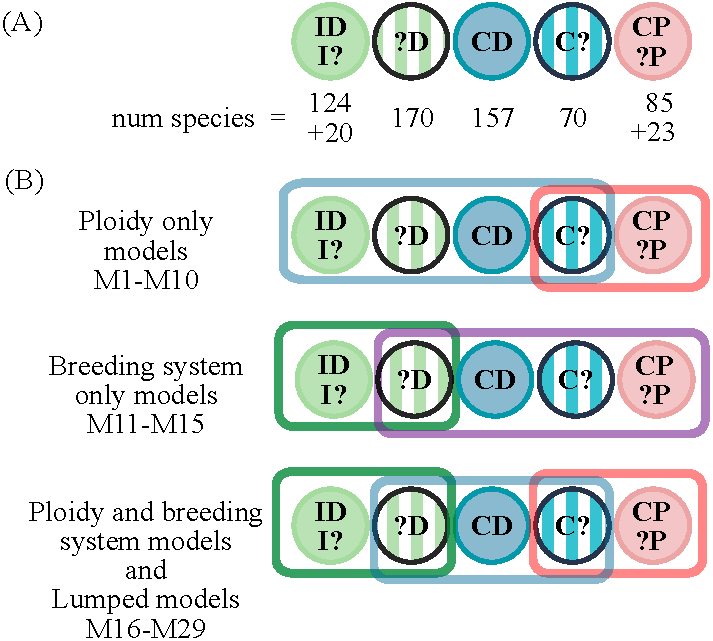
\includegraphics[width=0.5\textwidth]{states.pdf}
\caption{
Character states used for each of the models.
Each species retained on the tree belonged to one of five possible categories, depending on whether ploidy and/or breeding system were known. Character state abbreviations: $I$ for self-incompatible, $C$ for self-compatible, $D$ for diploid, $P$ for polyploid, $?$ for unknown.
(A) The five categories and the number of species in our data for each category.
Because polyploidization breaks this form of self-incompatibility, self-incompatible species with unobserved ploidy ($I?$) are taken to be diploid ($ID$), and polyploid species with unobserved breeding system ($?P$) are taken to be SC ($CP$).
(B) Category groupings into states for each model type.
For example, there are 70 species that are SC with unknown ploidy.
In the $D/P$ models these are coded as $D$ and $P$ (uncertain/consistent with either state), in the $I/C$ models they are coded as $C$, and in the $ID/CD/CP$ models they are coded as $CD$ and $CP$.
In the hidden state models, all species were coded as consistent with both $A$ and $B$.
Two species, \emph{Lycium californicum} and \emph{Solanum bulbocastanum}, are simultaneously $ID$ and $CP$, and by adding them the sample adds to the total of 651 taxa used for analyses.
}
\label{figure:stateclassifications}
\end{figure}

\begin{suppfigure}
    \caption{ All models.  [This figure is provided as a separate, large-format page.] }
    \label{fig:allmodels}
\end{suppfigure}


%%% Below here is old tables.  I think the new versions should instead go in results.tex or a separate file. %%%

% \begin{table}
% \begin{tabular}{lcccccc} \toprule
% \begin{tabular}{@{}lcccccc@{}} \toprule
%\multicolumn{4}{r}{Models} \\ \cmidrule(r){3-5}
%Model                     & Ploidy & Diploidization & Breeding  & Hidden & Num        & Marginal       \\
%                          &        &                & System    & State  & Parameters & Log-Likelihood \\ \midrule
%1. D/P                    & Yes    & No             & No        & No     & 5          & -1193.66\\
%2. D/P +$\delta$          & Yes    & Yes            & No        & No     & 6          & -1182.93 \\
%3. D/P+A/B                & Yes    & No             & No        & Yes    & 10         & -1150.99\\
%4. D/P+A/B+$\delta$       & Yes    & Yes            & No        & Yes    & 11         & \textbf{-1145.69}\\
%5. I/C                    & No     & No             & Yes       & No     & 5          & -1194.80 \\
%6. I/C+A/B                & No     & No             & Yes       & Yes    & 10         & \textbf{-1155.37}\\
%7. ID/CD/CP               & Yes    & No             & Yes       & No     & 9          & -1345.87\\
%8. ID/CD/CP+$\delta$      & Yes    & Yes            & Yes       & No     & 10         & -1344.50\\
%9. ID/CD/CP+A/B           & Yes    & No             & Yes       & Yes    & 15         & -1303.55 \\ 
%10. ID/CD/CP+A/B+$\delta$ & Yes    & Yes            & Yes       & Yes    & 16         & \textbf{-1300.35} \\
%\bottomrule
%\end{tabular}
%\caption{
   % The ten models and their marginal likelihoods.
    %Values in bold are for the best models within each class that are comparable (see \cref{table:}).
    %Abbreviations are D: diploid, P: polyploid, I: self-incompatible, C: self-compatible, A: one state of hidden trait, B: other state of hidden trait, $\delta$: diploidization.}
%\label{table:marginallike}
%\end{table}

\begin{table}
\addtolength{\tabcolsep}{-3pt}
\begin{tabular}{|l|r|c|c|c|c|l|}
\hline
Model                & \begin{tabular}[c]{@{}l@{}}Marginal\\ log-likelihood\end{tabular} & M2    & M3     & M4    & M5     & Evidence                                                                                     \\ \hline
M1. D/P              & -1283.76                                                          & 59.90 & 49.23  & 60.48 & 58.82  & \begin{tabular}[c]{@{}l@{}}Every model strongly \\ preferred over M1\end{tabular}            \\ \hline
\textbf{M2. CID D/P} & \textbf{-1223.86}                                                 &       & -10.66 & 0.579 & -1.079 & \begin{tabular}[c]{@{}l@{}}Strong preference for \\ M2 over M1\end{tabular}              \\ \hline
M3. D/P+A/B          & -1234.52                                                          &       &        & 11.24 & 9.58   & \begin{tabular}[c]{@{}l@{}}Asymmetric rates strongly\\ preferred over symmetric\end{tabular}   \\ \hline
\textbf{M4. D/P+A/B asym}     & \textbf{-1223.28}                                                          &       &        &       & -1.658 & \begin{tabular}[c]{@{}l@{}}Moderate evidence for\\ only asymmetric hidden rates\end{tabular} \\\hline
M5. D/P+A/B all asym & -1224.93                                                          &       &        &       &        &          \\ \hline                                                                                   
\end{tabular}
\caption{Bayes factors of  ploidy-only models without diplodization. Numbers greater that 1 mean moderate support relative to the model in the row label.  Conventional threshold for `strong' support is 10. The best models are written in bold. }
\label{table:bayesfactors}
\end{table}

% B: M111->M11
\begin{table}
\addtolength{\tabcolsep}{-3pt}
\begin{tabular}{|l|r|c|c|c|c|l|}
\hline
Model                      & \begin{tabular}[c]{@{}l@{}}Marginal\\ log-likelihood\end{tabular} & M12   & M13   & M14   & M15   & Evidence                                                                                       \\ \hline
M11. I/C                   & -1309.07                                                          & 41.13 & 38.59 & 61.34 & 61.40 & \begin{tabular}[c]{@{}l@{}}Every model strongly \\ preferred over M11\end{tabular}            \\ \hline
M12. CID I/C               & -1267.93                                                          &       & -2.53 & 20.21 & 20.37 & \begin{tabular}[c]{@{}l@{}}Models with asymmetric rates\\ are preferred over  M12\end{tabular} \\ \hline
M13. I/C+A/B               & -1270.47                                                          &       &       & 22.75 & 22.80 & \begin{tabular}[c]{@{}l@{}}Asymmetric rates strongly\\ preferred over symmetric\end{tabular}   \\ \hline
\textbf{M14. I/C+A/B asym} & \textbf{-1247.72}                                                 &       &       &       & 0.05 & No evidence                                                                                    \\ \hline
\textbf{M15. I/C+A/B all asym }     & \textbf{ -1247.66}                                                          &       &       &       &       &       \\ \hline                                                                                        
\end{tabular}
\caption{Bayes factors of breeding system-only models. Results indicate that the HiSSE models with asymmetric rates (M14, M15) are strongly preferred over every other model.}
\label{table:M11M15}
\end{table}

% E: Could we include a figure of the traits on the tree?  At least as supp info. FIXME
%B: "K=ln(BF(M1,M2))" -> "K=ln(BF($M_{i}$,$M_{ii}$))" because we use M1 and M2 for model names.
\begin{table}[]
\addtolength{\tabcolsep}{-3pt}
\begin{tabular}{|l|c|c|c|c|}
\hline
Model                       & \begin{tabular}[c]{@{}l@{}}Marginal\\ log-likelihood\end{tabular} & Comparison  & K=ln(BF($M_{i}$,$M_{ii}$)) & \begin{tabular}[c]{@{}l@{}}Preferred\\ Model (Evidence)\end{tabular} \\ \hline
M26. Lumped D/P             & -1463.22                                                          & M26 vs. M16 & 4.10            & M16 (Moderate)                                                       \\
\textbf{M16. ID/CD/CP}      & \textbf{-1459.11}                                                 &             &                 &                                                                      \\ \hline
M27. Lumped D/P+A/B         & -1417.67                                                          & M27 vs. M23 & 3.678           & M23 (Moderate)                                                       \\
\textbf{M23. ID/CD/CP +A/B} & \textbf{-1414.00}                                                 &             &                 &                                                                      \\ \hline
M28. Lumped I/C             & -1458.41                                                          & M28 vs. M16 & -0.69           & No evidence                                                          \\
\textbf{M16. ID/CD/CP}      & \textbf{-1459.11}                                                 &             &                 &                                                                      \\ \hline
M29. Lumped I/C+ A/B        & -1416.60                                                          & M29 vs. M23 & 2.60            & M23 (Moderate)                                                       \\
\textbf{M23. IC/CD/CP+A/B}  & \textbf{-1414.00}                                                 &             &                 &                                                                      \\ \hline
\end{tabular}
\caption{Test for adding a focal trait to a binary state model via Bayes factors. Three-state models are moderately preferred over two-state models. The evidence is stronger towards the inclusion of breeding systems in ploidy models (M26, M27) than the inclusion of ploidy in breeding system models (M29, M29)}
\label{table:lumped}
\end{table}

\begin{figure}
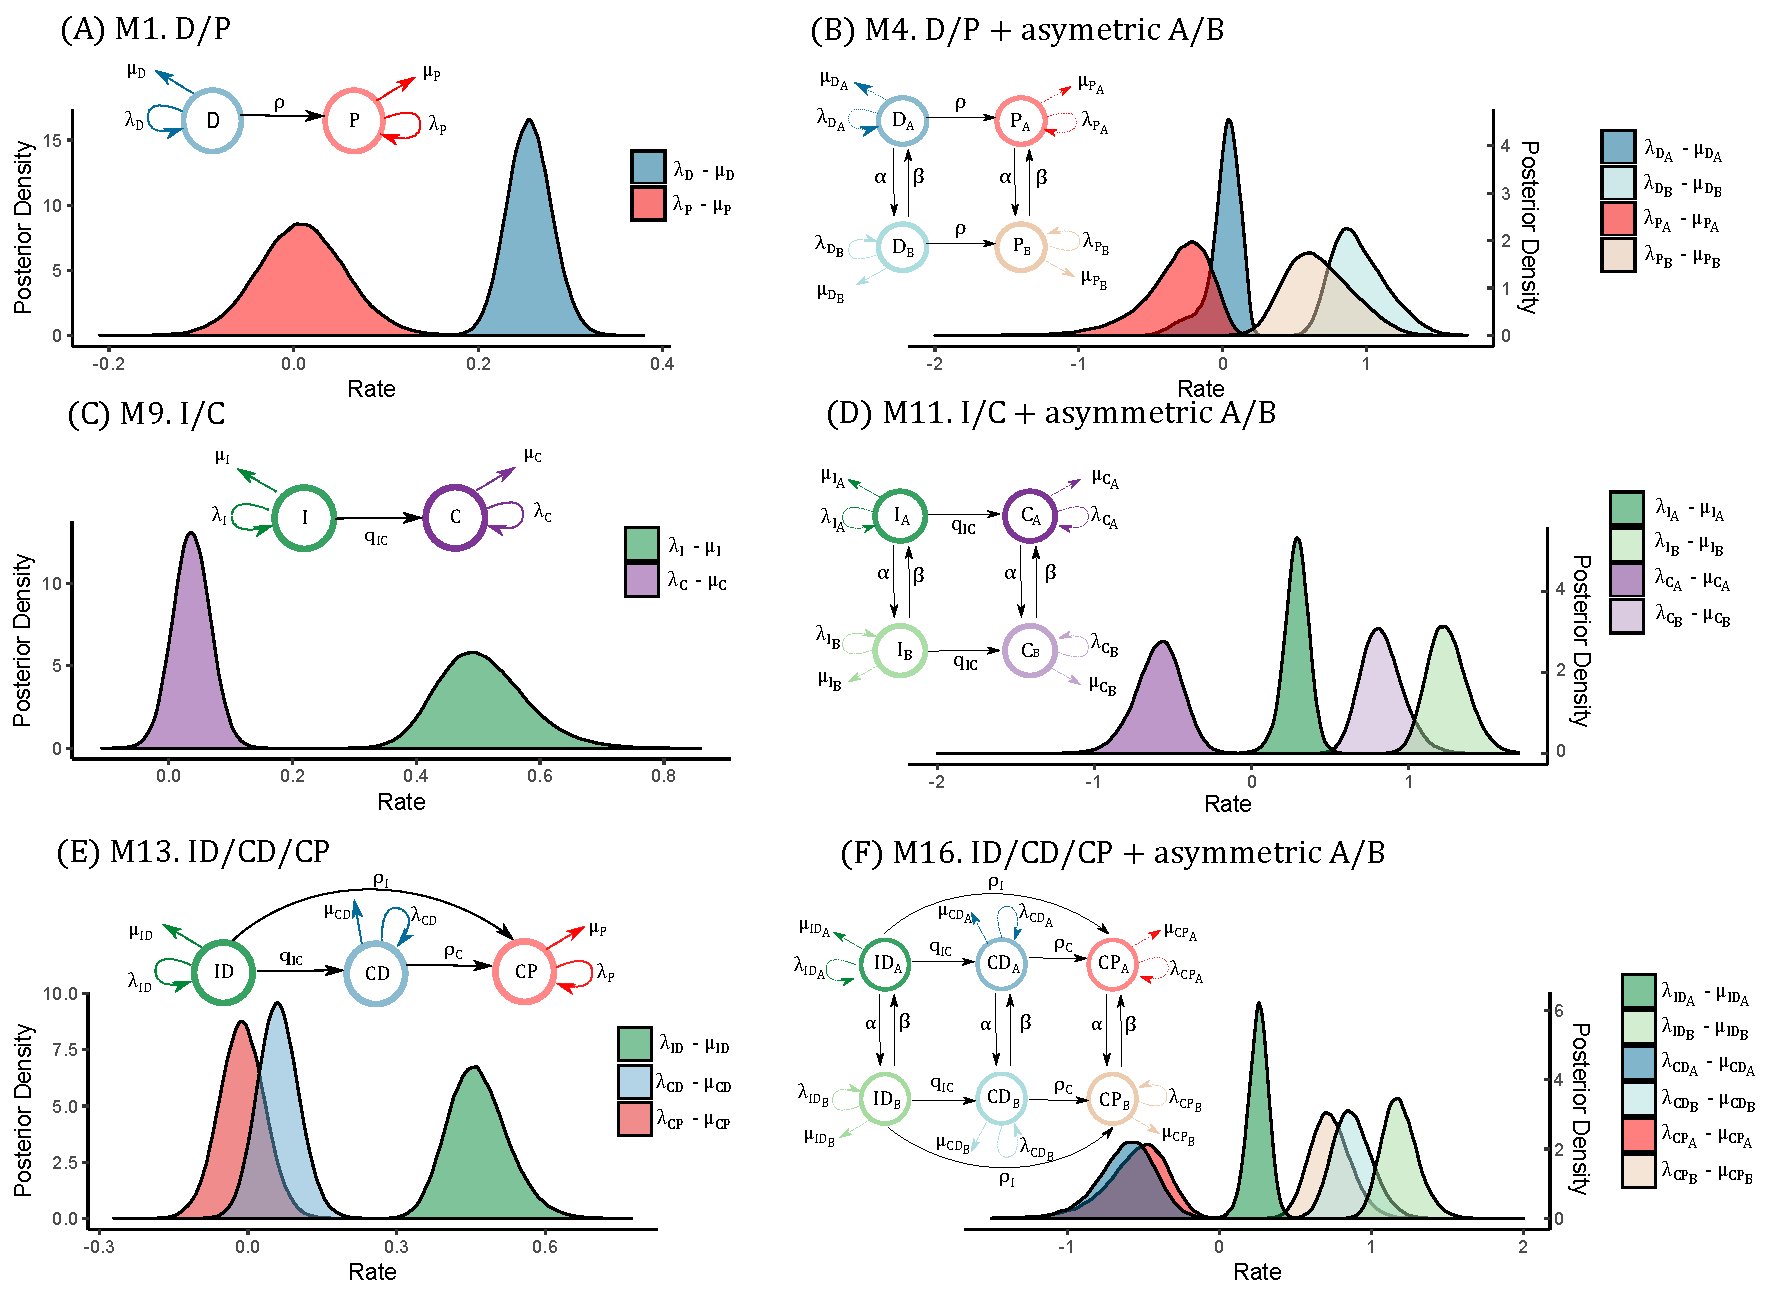
\includegraphics[width=\textwidth]{alldiversificationasymhidden.pdf} 
\caption{Net diversification rates for all models without diploidization rate estimate. 
Each panel contains a graphical summary of estimated model parameters and displays posterior distributions for net diversification estimates.}
\label{figure:netdivall}
\end{figure}

\begin{figure}
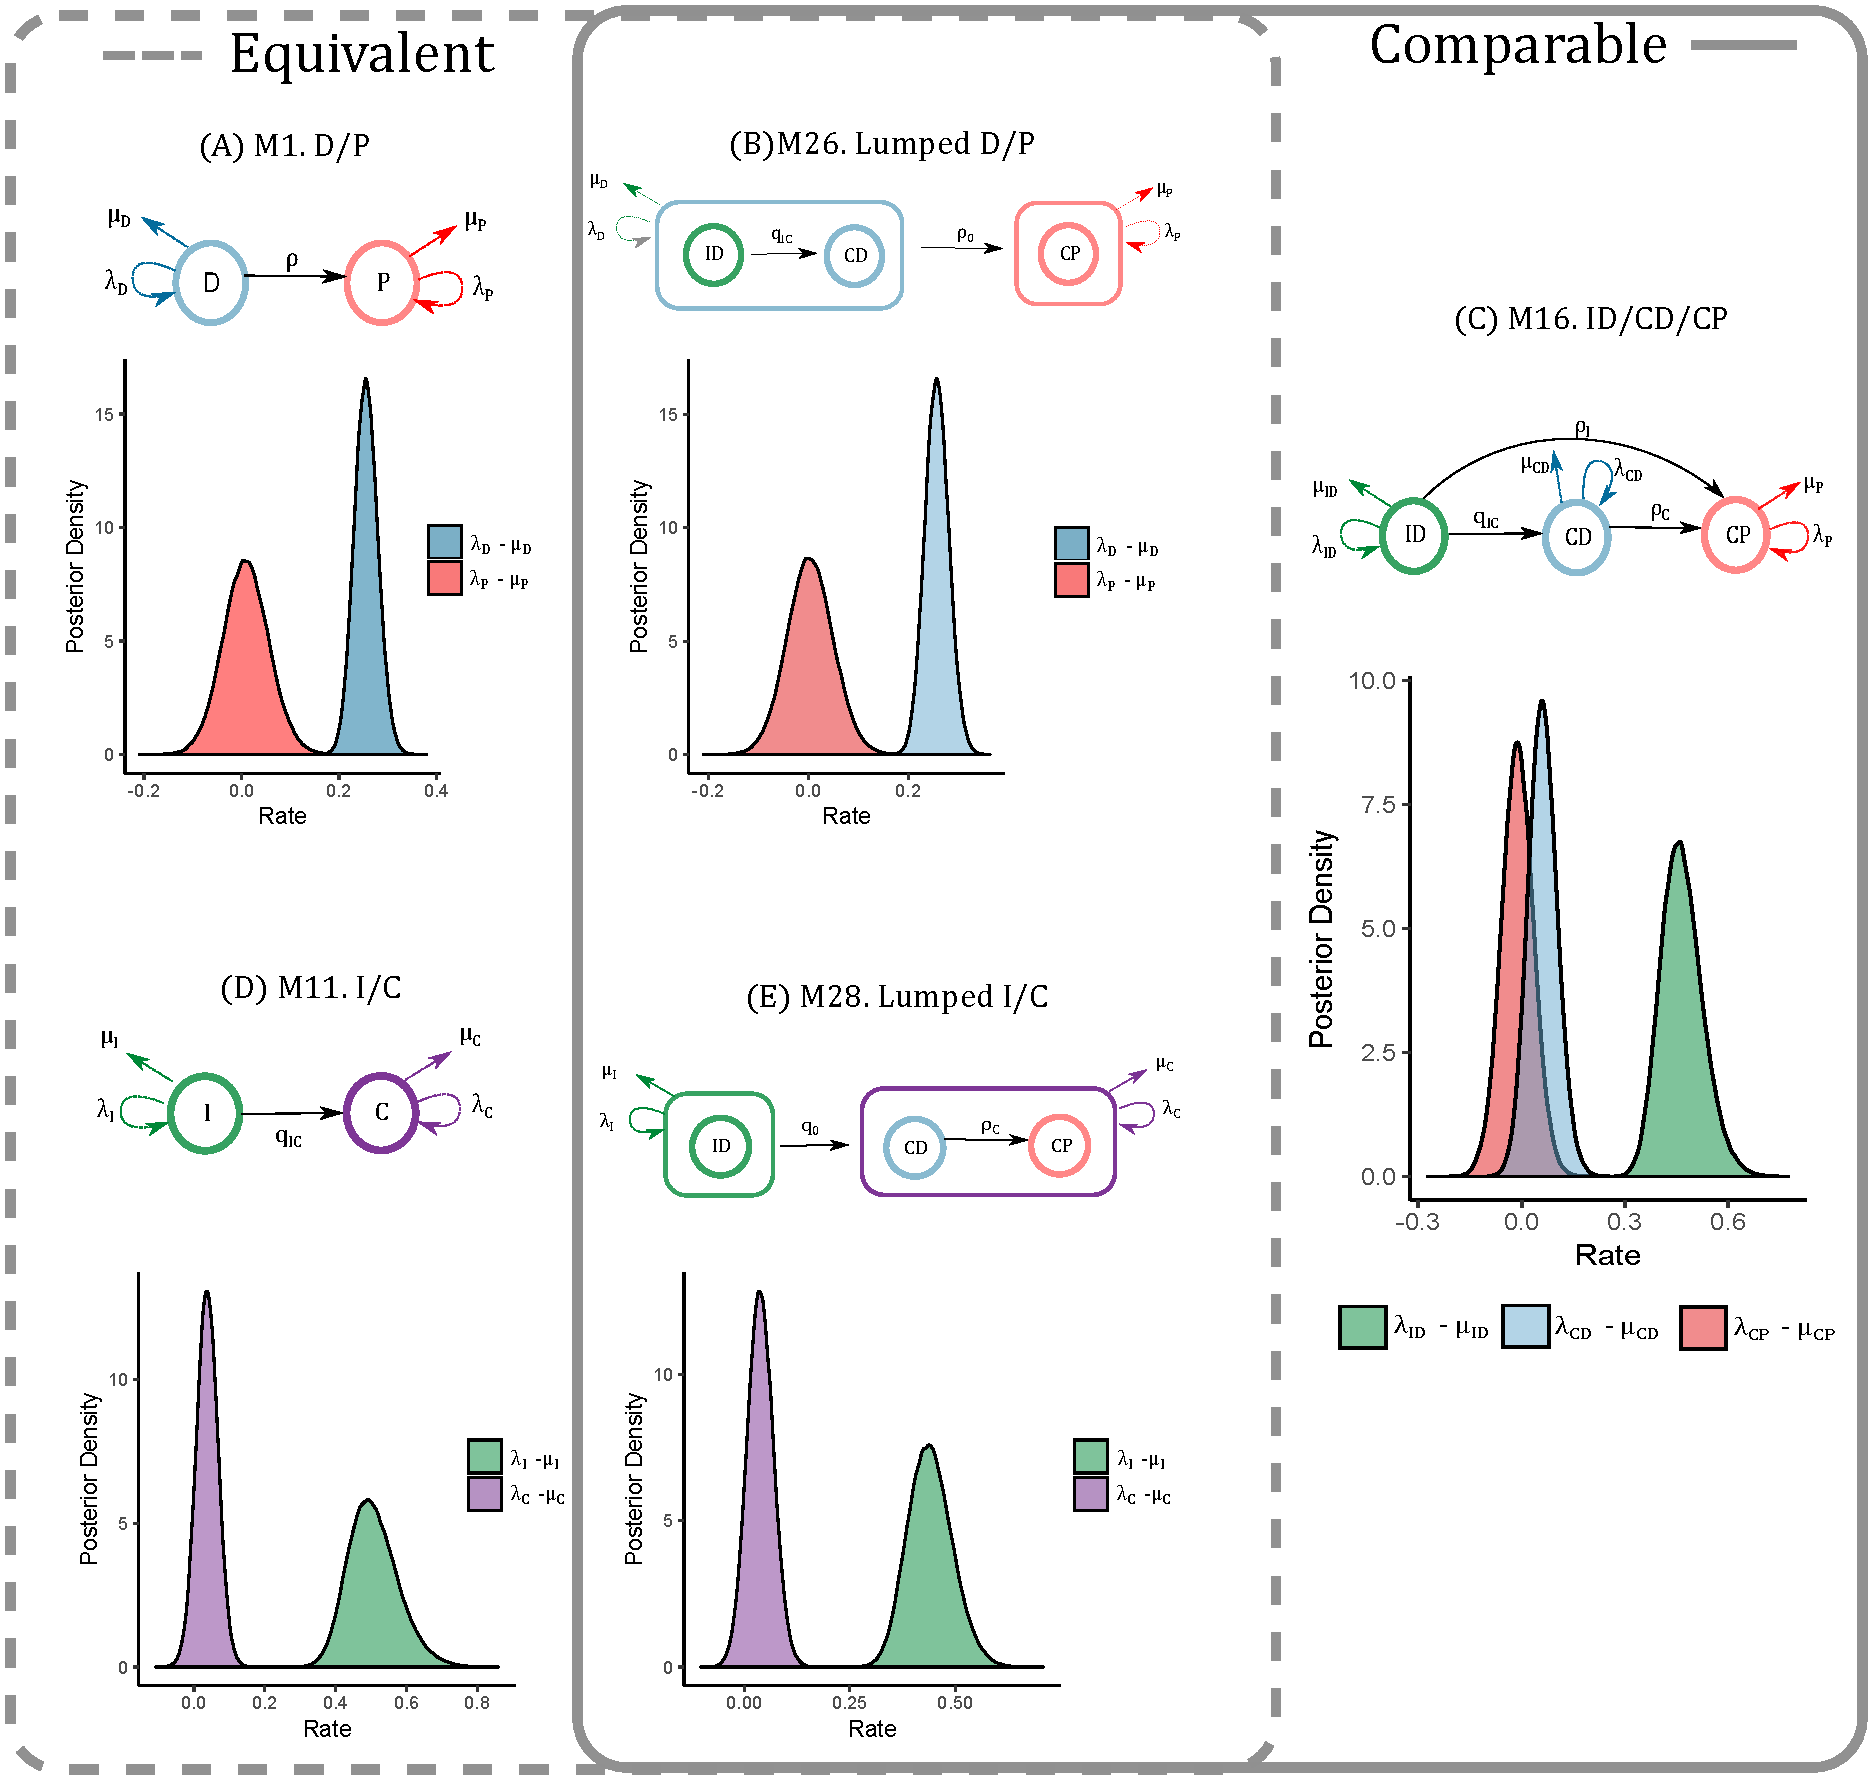
\includegraphics[width=\textwidth]{lumped.pdf} %lumped.pdf
\caption{Comparing two and three state models is possible via lumpable models (M26, M28). These models used the same classifications as the three-state model M16 which allow for comparisons via Bayes Factors as shown in \cref{table:lumped}.}  
\label{figure:lumped}
\end{figure}

% E todo: re-run with new rate estimates; add panel letters?
\begin{figure}
    \centering 
    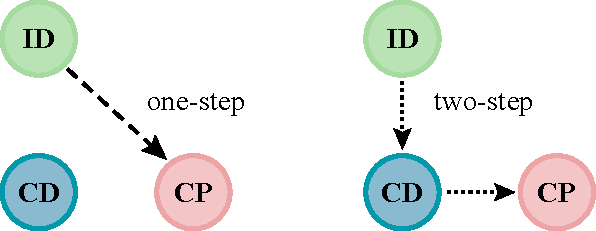
\includegraphics[width=0.5\textwidth]{pathstates2} \\ [40pt] 
        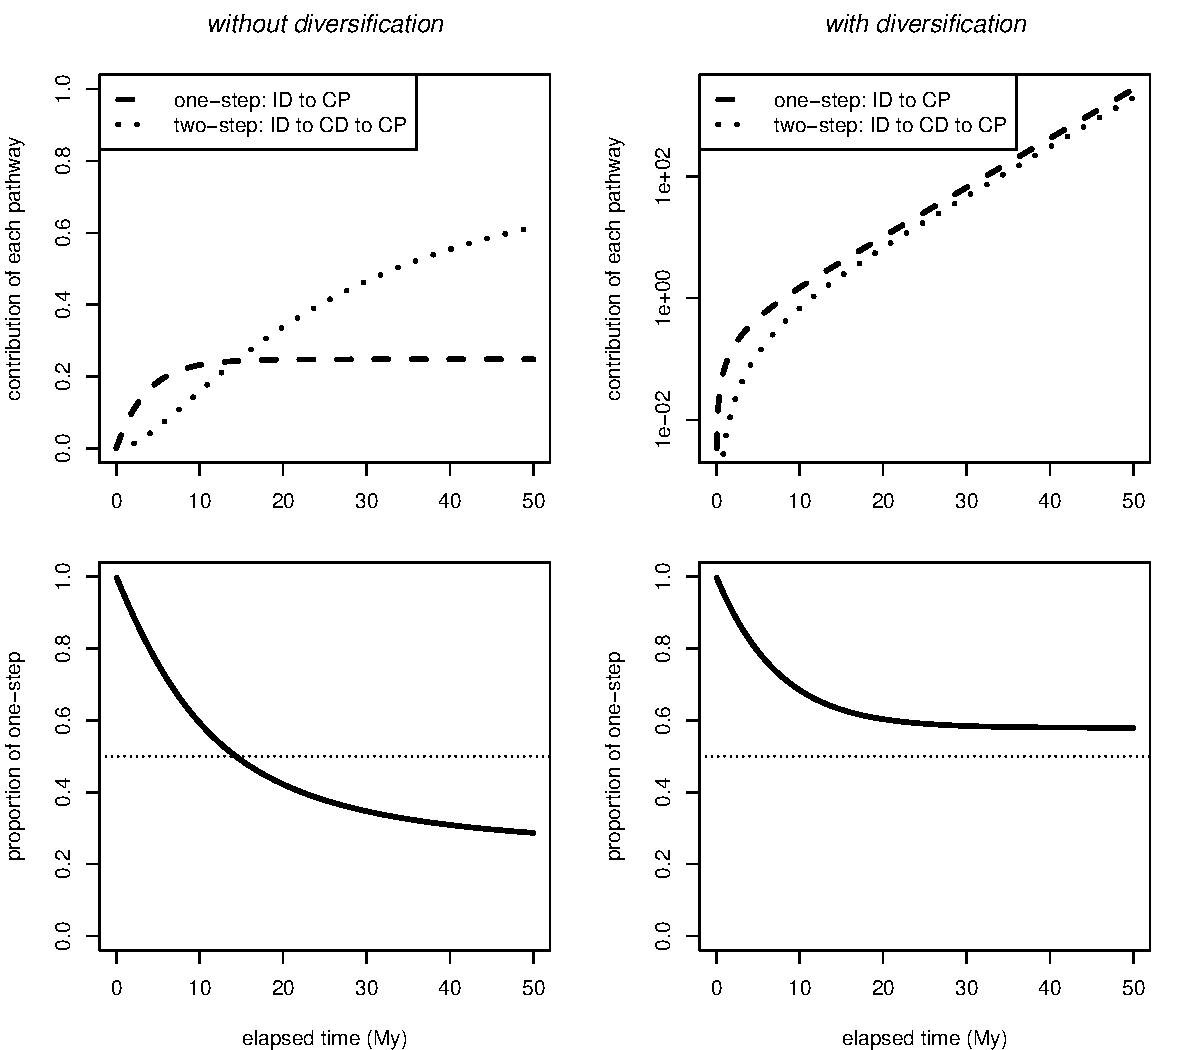
\includegraphics[width=0.9\textwidth]{pathways}
    \caption{
        Contributions of the two pathways to polyploidy.
        The one-step pathway is direct ID$\rightarrow$CP transitions.
        The two-step pathway consists of ID$\rightarrow$CD$\rightarrow$CP transitions.
        When considering only rates of transitions among the states (ignoring the diversification rate parameters), the one-step pathway dominates on short timescales and the two-step on long timescales (left panels).
        When also considering diversification within each state, the one-step pathway, in which polyploidization breaks down SI, dominates over any timescale (right panels).
        The top panels show the separate contributions of each pathway.
        The bottom panels show the proportional contribution of the one-step pathway (\ie one-step / [one-step + two-step]).
    }
    \label{figure:pathways}
\end{figure}


\begin{supptable}
\addtolength{\tabcolsep}{-3pt}
\begin{tabular}{|l|r|c|c|c|c|l|}
\hline
Model                           & \begin{tabular}[c]{@{}l@{}}Marginal\\ log-likelihood\end{tabular} & M7    & M8     & M9    & M10   & Evidence                                                                                     \\ \hline
M6. D/P+$\delta$                & -1268.83                                                          & 55.41 & 42.78  & 53.37 & 52.85 & \begin{tabular}[c]{@{}l@{}}Every model strongly \\ preferred over M6\end{tabular}            \\ \hline
\textbf{M7. CID D/P+$\delta$}   & \textbf{-1212.42}                                                 &       & -12.62 & -2.04 & -2.04 & \begin{tabular}[c]{@{}l@{}}Model M7 moderately\\ preferred over M9 and M10\end{tabular}      \\ \hline
M8. D/P+A/B $\delta$            & -1214.46                                                          &       &        & 10.58 & 10.07 & \begin{tabular}[c]{@{}l@{}}Asymmetric rates strongly\\ preferred over symmetric\end{tabular} \\ \hline
M9. D/P+A/B +$\delta$ asym      & -1214.46                                                          &       &        &       & -0.51 & No evidence                                                                                  \\ \hline
M10. D/P+A/B +$\delta$ all asym & -1214.97                                                          &       &        &       &       &         \\ \hline                                                                                    
\end{tabular}
\caption{Bayes factors of  ploidy-only models with diplodization. Results indicate that a character independent model (M6) is strongly preferred over BiSSE (M1)  model. M6 is moderately preferred over any of the HiSSE models with asymmetric hidden rates (M9, M10).}
\label{supptable:M6M10}
\end{supptable}

\begin{supptable}
\addtolength{\tabcolsep}{-3pt}
\begin{tabular}{|l|r|c|c|c|c|l|}
\hline
Model                            & \begin{tabular}[c]{@{}l@{}}Marginal\\ log-likelihood\end{tabular} & M18   & M19   & M20   & Evidence                                                                                                   \\ \hline
M16. ID/CP/CD                    & -1459.11                                                          & 45.11 & 65.91 & 63.98 & \begin{tabular}[c]{@{}l@{}}Every model strongly \\ preferred over M16\end{tabular}                         \\ \hline
M17. CID ID/CP/CD                & *                                                                 &       &       &       &                                                                                                            \\
M18. ID/CP/CD+A/B                & -1414                                                             &       & 20.79 & 18.87 & \begin{tabular}[c]{@{}l@{}}Asymmetric rates strongly\\ preferred over symmetric\end{tabular}               \\ \hline
\textbf{M19. ID/CP/CD +A/B asym} & \textbf{-1393.20}                                                 &       &       & -1.92 & \begin{tabular}[c]{@{}l@{}}Asymmetric hidden rates moderately\\ preferred over all asymmetric\end{tabular} \\ \hline
M20. ID/CP/CD +A/B all asym      & -1393.12                                                          &       &       &       &   \\ \hline                                                                                                        
\end{tabular}
\caption{Bayes factors of ploidy and breeding system withou diploidization. Results indicate that the MuHiSSE model with asymmetric hidden rates (17) is  strongly preferred over M16 and M18 and moderately preferred over the MuHiSSe with all rates asymetric (M20). *Marginal log-likelihood for M17 could not be calculated within allotted computer time.}
\label{supptable:M16M20}
\end{supptable}

\begin{supptable}
\addtolength{\tabcolsep}{-3pt}
\begin{tabular}{|l|r|c|c|c|c|l|}
\hline
Model                                 & \begin{tabular}[c]{@{}l@{}}Marginal\\ log-likelihood\end{tabular} & M22   & M23    & M24   & M25   & Evidence                                                                                         \\ \hline
M21. ID/CP/CD+$\delta$                & -1454.68                                                          & 55.48 & 46.031 & 67.94 & 65.15 & \begin{tabular}[c]{@{}l@{}}Every model strongly \\ preferred over M21\end{tabular}               \\ \hline
M22. CID ID/CP/CD+$\delta$            & -1399.201                                                         &       & -9.452 & 12.45 & 9.675 & \begin{tabular}[c]{@{}l@{}}Model M24 strongly preferred \\ over M22\end{tabular}                 \\ \hline
M23. ID/CP/CD+A/B $\delta$            & -1408.65                                                          &       &        & 21.91 & 19.12 & \begin{tabular}[c]{@{}l@{}}Asymmetric rates strongly\\ preferred over symmetric\end{tabular}     \\ \hline
\textbf{M24. ID/CP/CD +$\delta$ asym} & \textbf{-1386.74}                                                 &       &        &       & -2.78 & \begin{tabular}[c]{@{}l@{}}Asymmetric hidden rates \\ preferred over all asymmetric\end{tabular} \\ \hline
M25. ID/CP/CD +$\delta$ all asym      & -1389.52                                                          &       &        &       &       &                      \\ \hline                                                                           
\end{tabular}
\caption{Bayes factors of ploidy and breeding system with diploidization. Results indicate that the MuHiSSE model with asymmetric hidden rates (M24) is  strongly preferred over M21-M23 and moderately preferred over the MuHiSSe with all rates asymmetric (M25).}
\label{supptable:M21M25}
\end{supptable}

\begin{supptable}
\addtolength{\tabcolsep}{-5pt}
\begin{tabular}{|l|c|c|c|c|}
\hline
Model                                    & \begin{tabular}[c]{@{}l@{}}Marginal\\ log-likelihood\end{tabular} & Comparison  & K=log(BF(M1,M2) & \begin{tabular}[c]{@{}l@{}}Preferred\\ Model (Evidence)\end{tabular} \\ \hline
M1. D/P                                  & -1238.76                                                          & M1 vs. M4   & 60.47           & M4 (Strong)                                                          \\
\textbf{M4. D/P+A/B asym}                & \textbf{-1223.28}                                                &             &                 &                                                                      \\ \hline
M11. I/C                                 & -1309.07                                                          & M11 vs. M14 & 61.35           & M14 (Strong)                                                         \\
\textbf{M14. I/C+A/B asym}               & \textbf{-1247.72}                                                 &             &                 &                                                                      \\ \hline
M16. ID/CD/CP                            & -1459.11                                                          & M16 vs. M19 & 65.90           & M19 (Strong)                                                         \\
\textbf{M19. ID/CD/CP+A/B asym}          & \textbf{-1393.20}                                                &             &                 &                                                                      \\ \hline
M6. D/P+$\delta$                         & -1283.76                                                          & M6 vs. M9   & 69.3            & M9 (Strong)                                                          \\
\textbf{M9. D/P+A/B+$\delta$ asym}       & \textbf{-1214.46}                                                 &             &                 &                                                                      \\ \hline
M21. IC/CD/CP+$\delta$                   & -1454.68                                                          & M21 vs. M24 & 68.48           & M24 (Strong)                                                         \\
\textbf{M24. IC/CD/CP+A/B+$\delta$ asym} & \textbf{-1386.20}                                                 &             &                 &                                                                      \\ \hline
\end{tabular}
\caption{Test for addition of hidden states in models via Bayes factors. Models with hidden states are strongly preferred over simpler models}
\label{supptable:testaddhidden}
\end{supptable}

\begin{supptable}
\addtolength{\tabcolsep}{-3pt}
\begin{tabular}{|l|c|c|c|c|}
\hline
Model                                    & \begin{tabular}[c]{@{}l@{}}Marginal\\ log-likelihood\end{tabular} & Comparison  & K=log(BF(M1,M2) & \begin{tabular}[c]{@{}l@{}}Preferred\\ Model (Evidence)\end{tabular} \\ \hline
M1. D/P                                  & -1238.76                                                          & M1 vs. M6   & 65.92           & M6 (Strong)                                                          \\
\textbf{M6. D/P+$\delta$}                & \textbf{-1267.84}                                                 &             &                 &                                                                      \\ \hline
M4. D/P+A/B asym                         & -1223.28                                                          & M4 vs. M9   & 8.81            & M9 (Moderate)                                                        \\
\textbf{M9. D/P+A/B+$\delta$ asym}       & \textbf{-1214.46}                                                 &             &                 &                                                                      \\ \hline
M16. ID/CD/CP                            & -1459.11                                                          & M16 vs. M21 & 4.41            & M21 (Moderate)                                                       \\
\textbf{M21. ID/CD/CP+$\delta$}          & \textbf{-1454.68}                                                 &             &                 &                                                                      \\ \hline
M19. IC/CD/CP asym                       & -1393.20                                                          & M19 vs. M24 & 6.46            & M24 (Moderate)                                                       \\
\textbf{M24. IC/CD/CP+A/B+$\delta$ asym} & \textbf{-1386.20}                                                 &             &                 &                                                                      \\ \hline
\end{tabular}
\caption{Test for inclusion of a diploidization rate via Bayes factors. Models with diploidization are moderately preferred over models that do not include a diploidization rate}
\label{supptable:testdiploidization}
\end{supptable}


\begin{supptable}
\addtolength{\tabcolsep}{-5pt}
\begin{tabular}{|l|c|c|c|l|}
\hline
Model                                    & \begin{tabular}[c]{@{}l@{}}Marginal\\ log-likelihood\end{tabular} & Comparison  & K=log(BF(M1,M2) & \begin{tabular}[c]{@{}l@{}}Preferred\\ Model (Evidence)\end{tabular} \\ \hline
M3. D/P+A/B                                 & -1234.52                     &    M3 vs. M4                 & 11.239                  & M4 (Strong)   \\
\textbf{M4. D/P+ A/B asym}            & -1223.28                     &   M4 vs. M5              & -1.658                  & M4 (Moderate)   \\
M5. D/P+A/B all asym                 & -1224.93                     &                     &                         &                         \\ \hline
M13. I/C+ A/B                                & -1270.47                     &   M13 vs. M14                  & 22.75                   & M14 (Strong)   \\
\textbf{M14. I/C+ A/B asym}            & \textbf{-1247.72}            & M14 vs. M15         & {0.05}           & No evidence             \\
M15. I/C+ A/B all asym               & -1247.67                     &                     &                         &                         \\ \hline
M18. IC/CD/CP+A/B                            & -1414.00                     &     M18 vs. M19                & 20.79                   & M19 (Strong)    \\
\textbf{M19. IC/CD/CP+ A/B asym}       & \textbf{-1393.21}            & M19 vs. M20          & {-1.919}         & M19 (Moderate)   \\
M20. IC/CD/CP+ A/B all asym           & -1395.129                    &                     &                         &                         \\ \hline
M8. D/P +A/B+$\delta$                          & -1225.05                     &  M8 vs. M9                   & 10.58                   & M9 (Strong)    \\
\textbf{M9. D/P+ A/B+ $\delta$ asym}      & \textbf{-1214.46}                     &    M9 vs. M10                 & -0.52                   & M10 (Moderate) \\
M10. D/P+A/B+$\delta$ all asym        & -1214.98                     &                    &                         &                         \\ \hline
M23. IC/CD/DP+A/B+$\delta$                 & -1408.65                     &     M23 vs M24                & 21.91                   & M24(Strong)     \\
\textbf{M24. IC/CD/DP+A/B+$\delta$ asym} & \textbf{-1386.74}                     &   M24 vs M25              & -2.78                   & M24 (Moderate) \\
M25. IC/CD/DP+A/B+ $\delta$ all asym     & -1389.52                     &                     &                         &                         \\ \hline
\end{tabular}
\caption{Test for symmetry of the hidden and trait rates via Bayes factors. For all models asymmetric hidden transition rates are preferred over models with equal hidden rates. Adding more complexity by assuming asymmetry in the trait rate within hidden states does not improve models.}
\label{supptable:asymmetry}
\end{supptable}

% check values of delta and rho D/P+A/B with(out) delta
% i.e. parameter values in figure S1 & S4 vs Table S2

%B: heads up: I added two clarifying descriptive sentences in the two figures below. Maybe something about noting x-axis scale differences would be useful.


\begin{suppfigure}
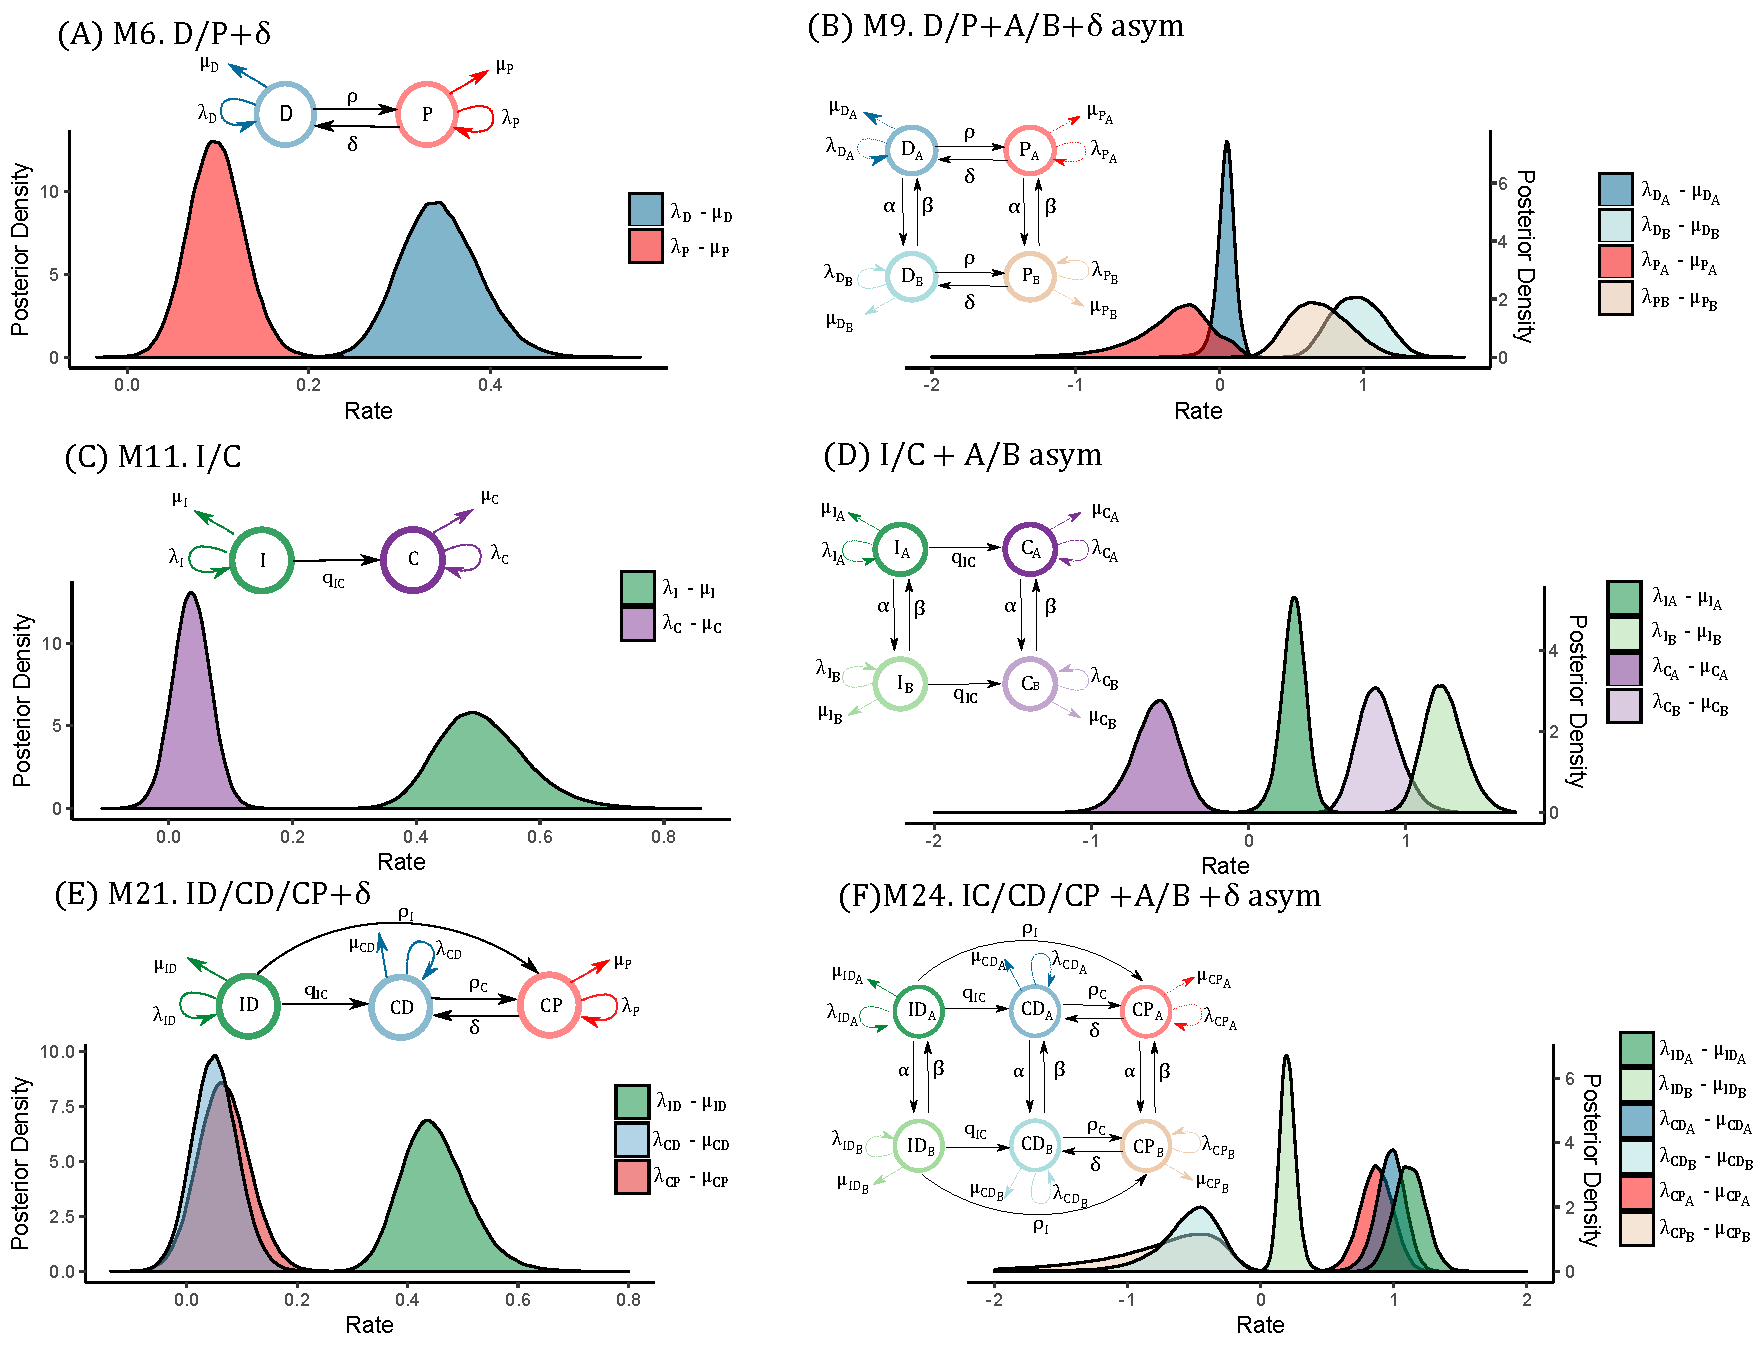
\includegraphics[width=\textwidth]{alldiversificationasymhiddendip.pdf}
\caption{Posterior distribution for all the best models with diploidization} % XXX
\label{suppfigure:alldip}
\end{suppfigure}

\begin{suppfigure}
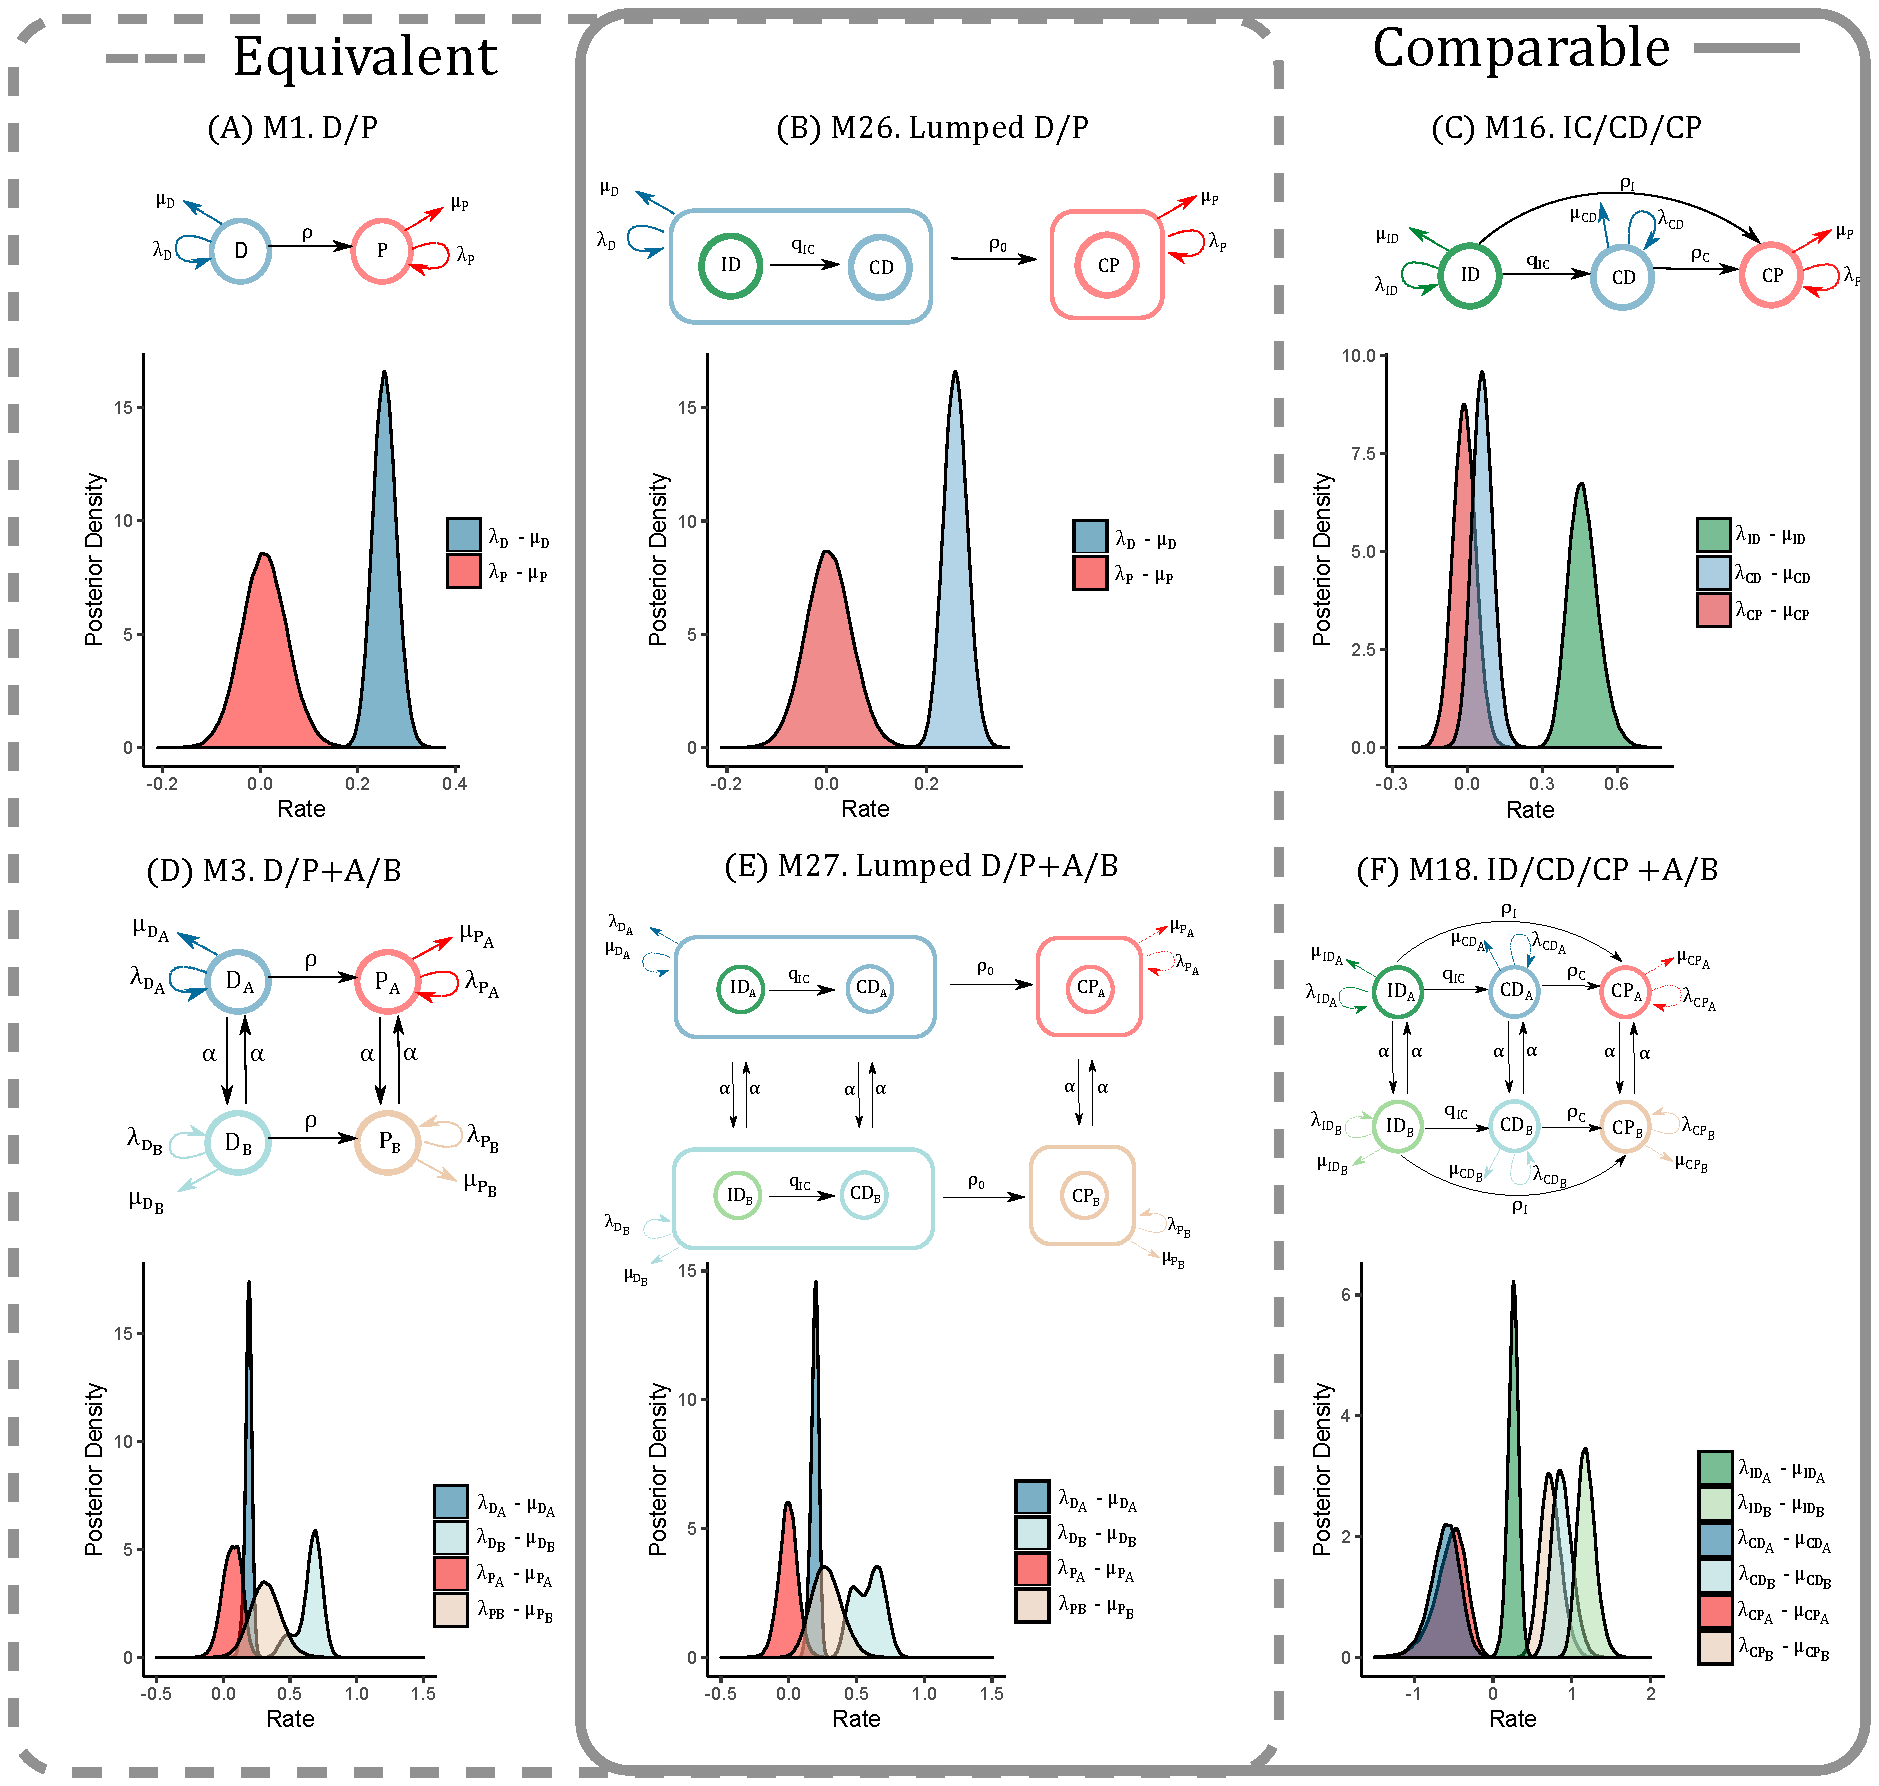
\includegraphics[width=\textwidth]{comparablesDP.pdf}
\caption{Lumped ploidy models to assess the effect of adding breeding system to create a three-state model. Moderate evidence exists that adding a breeding system is necessary \cref{table:lumped} } % XXX
\label{suppfigure:lumpedDP}
\end{suppfigure}

\begin{suppfigure}
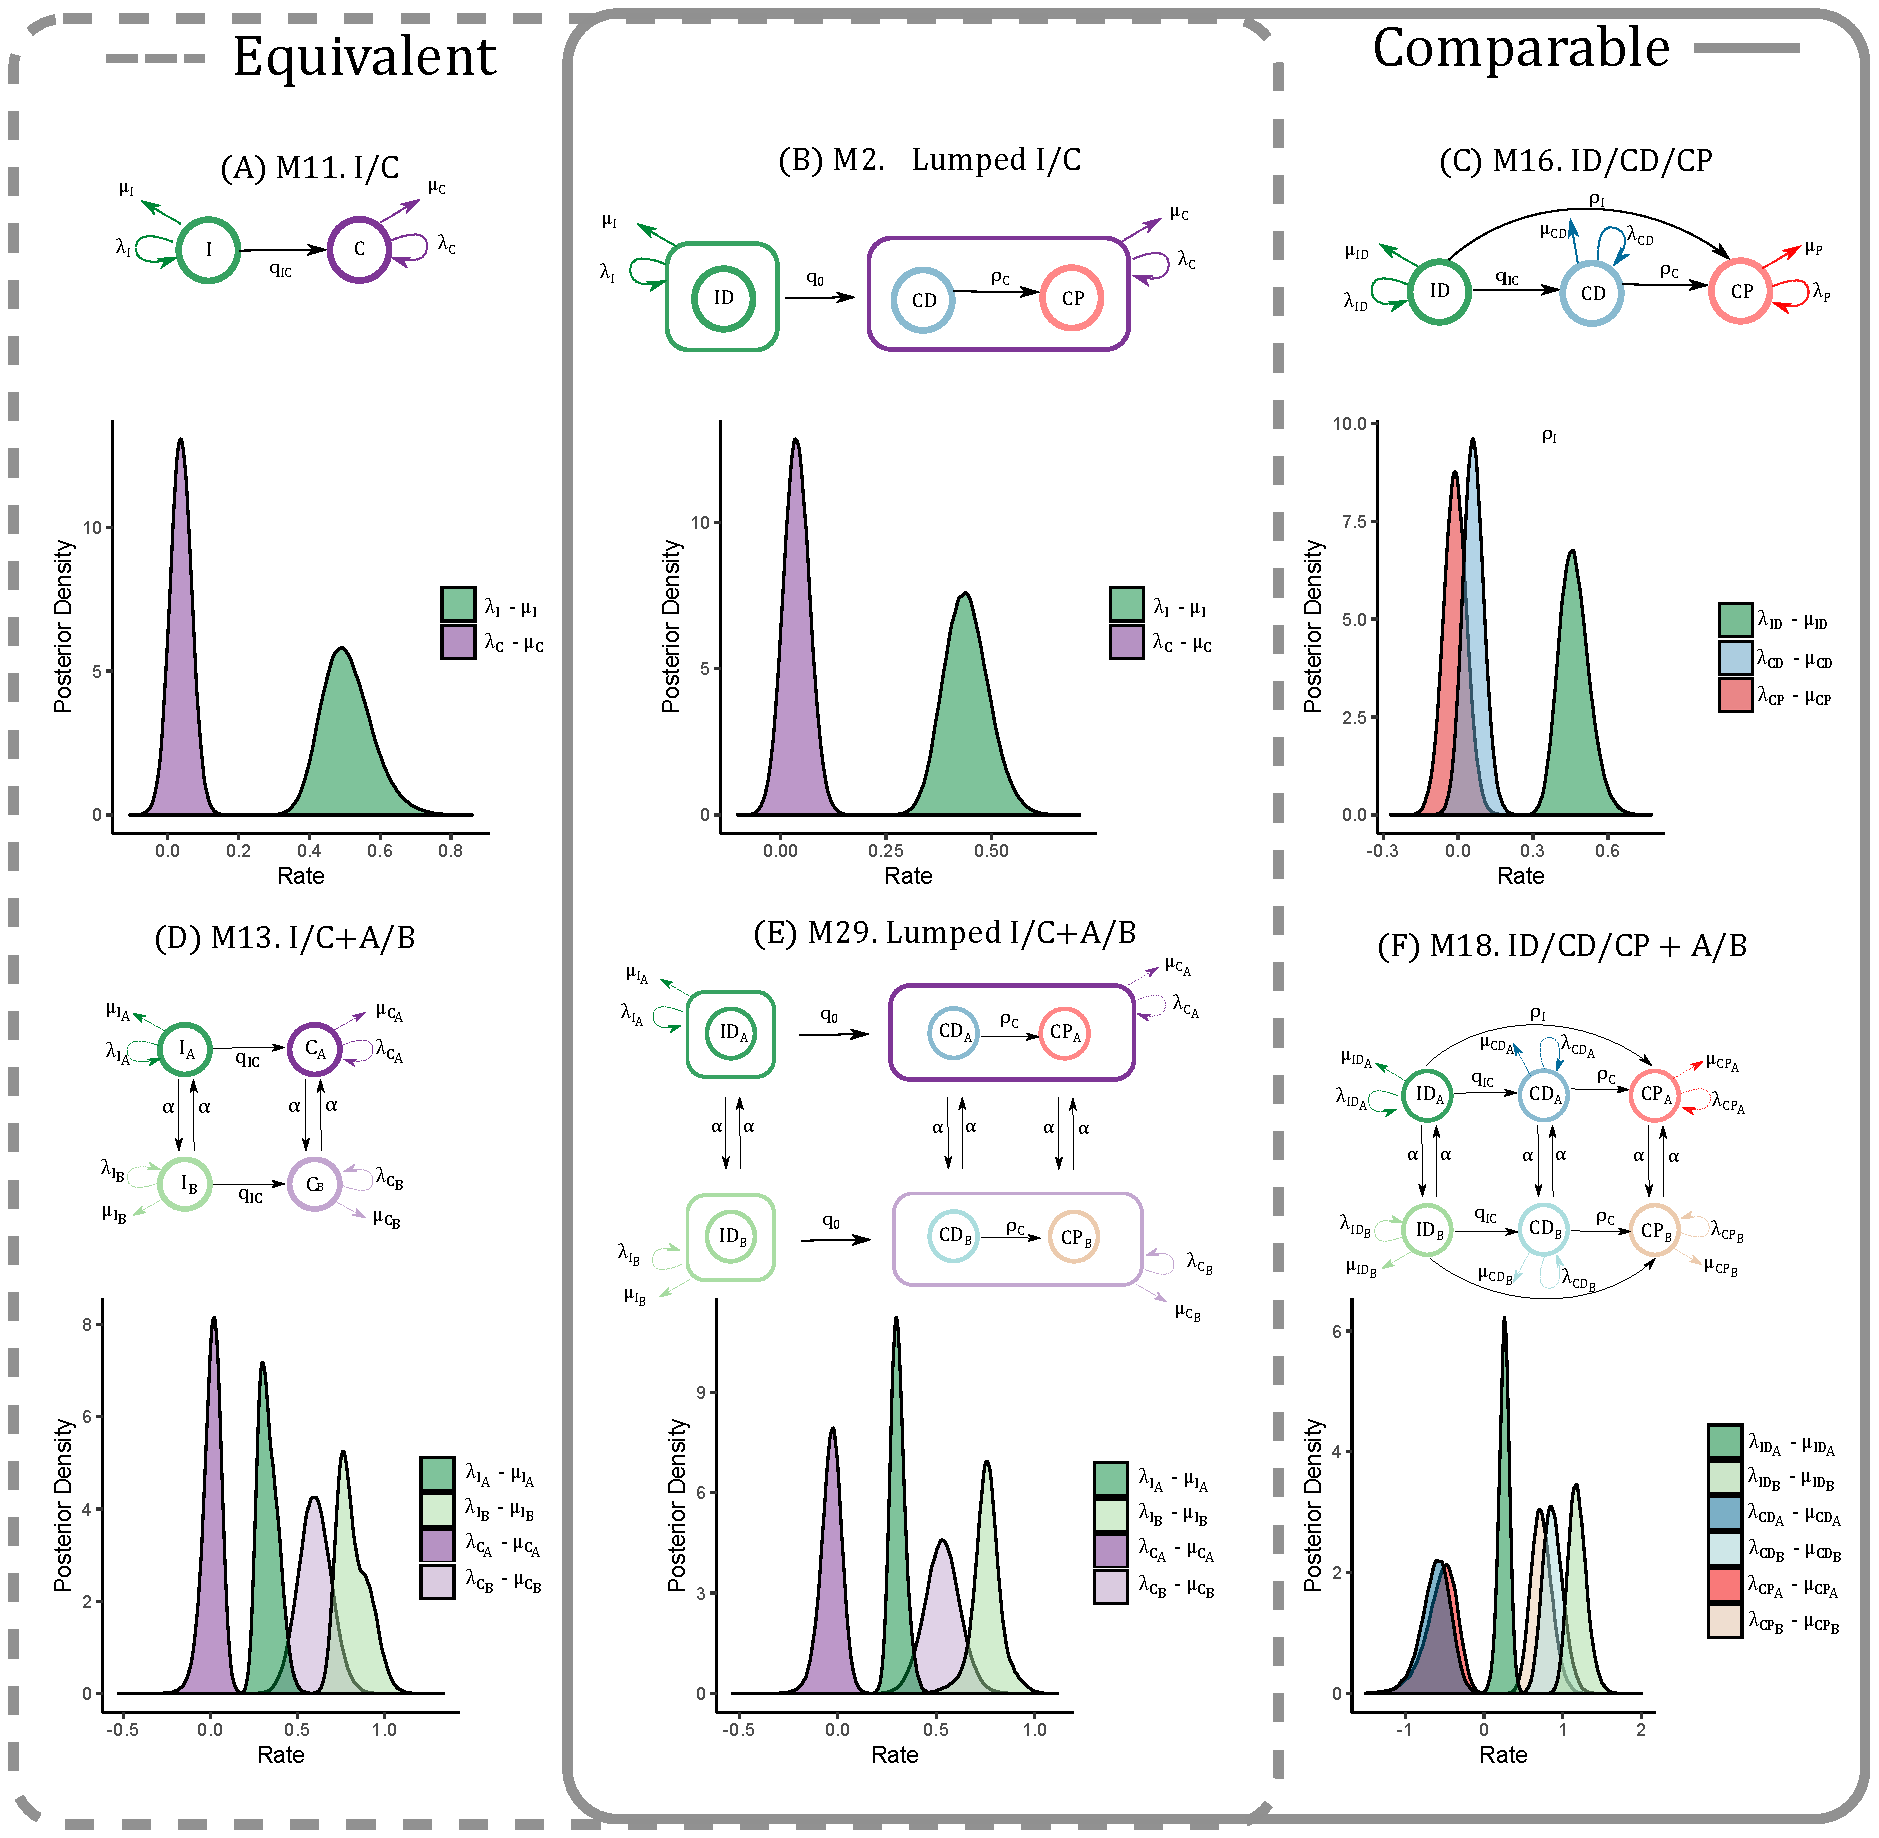
\includegraphics[width=\textwidth]{comparablesIC.pdf}
\caption{Lumped breeding system models to assess the effect of adding ploidy to create a three-state model. Moderate to insignificant evidence exists that adding ploidy is necessary \cref{table:lumped} } % XXX
\label{suppfigure:lumpedIC}
\end{suppfigure}


\begin{suppfigure}
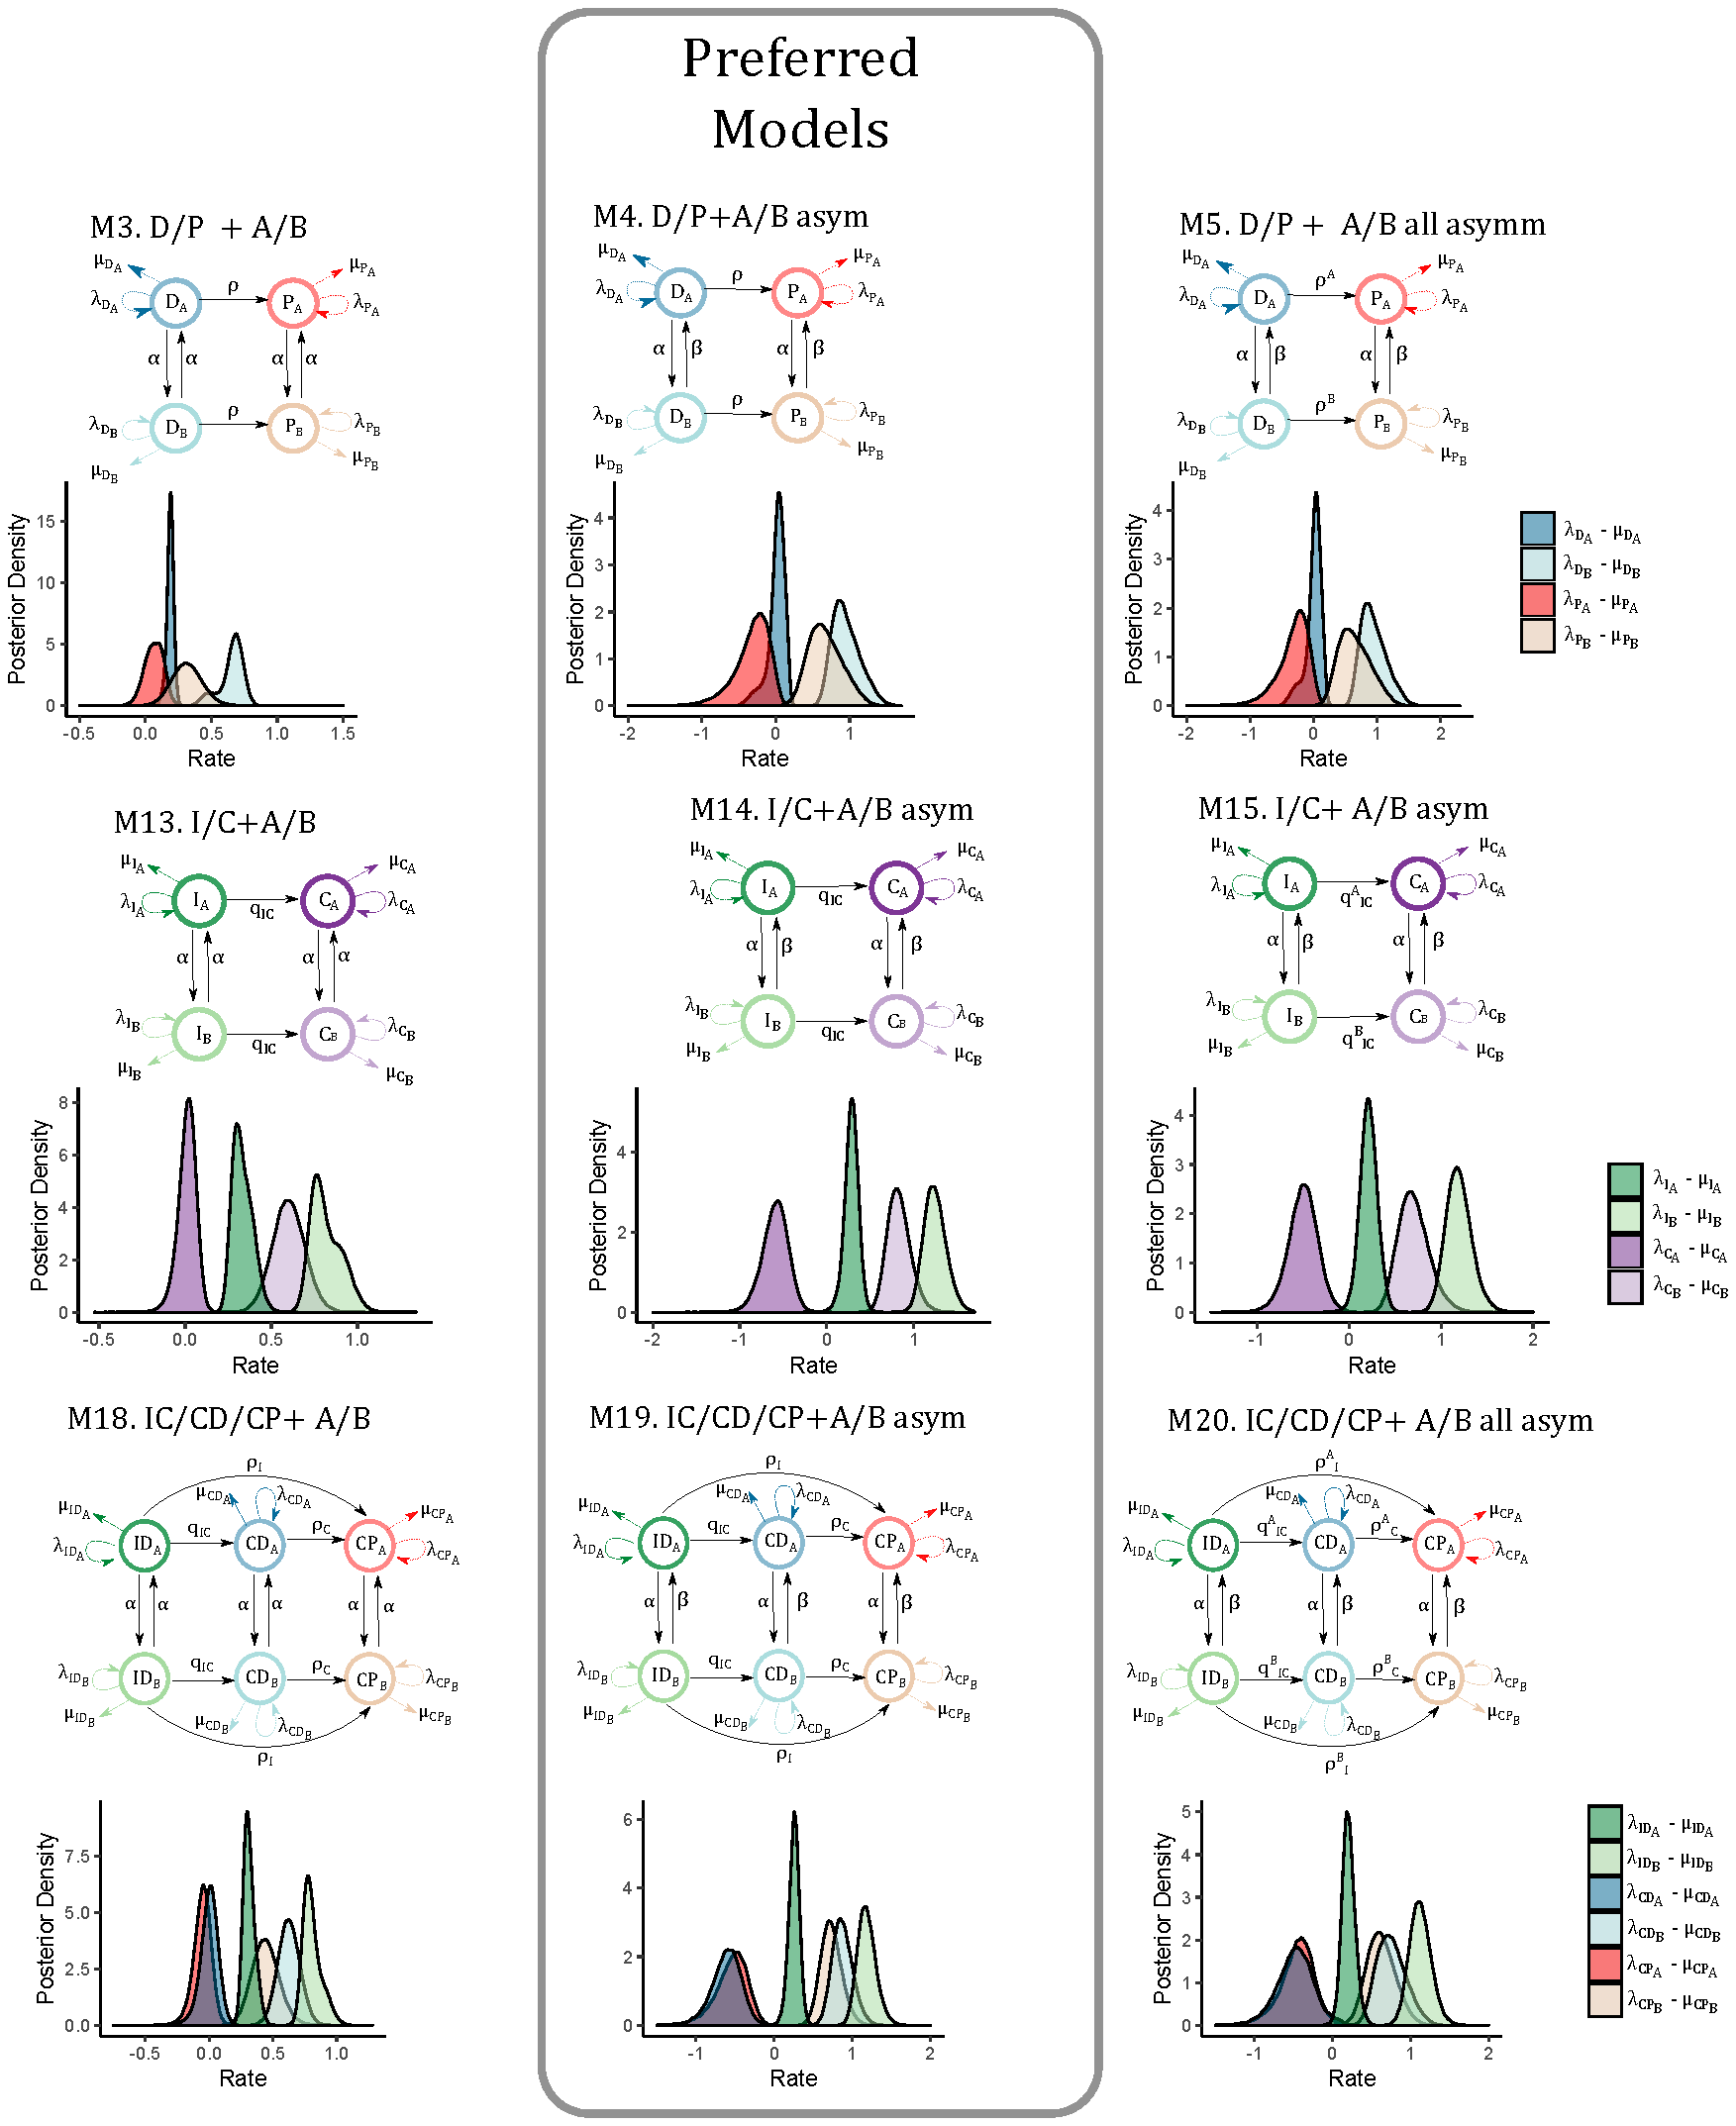
\includegraphics[width=\textwidth]{effectofasymmetry.pdf}
\caption{Effect of asymmetric rates in hidden models. Models with asymmetric rates are preferred over models with equal rates \cref{supptable:asymmetry}} % XXX
\label{suppfigure:asymmetric}
\end{suppfigure}


\begin{suppfigure}
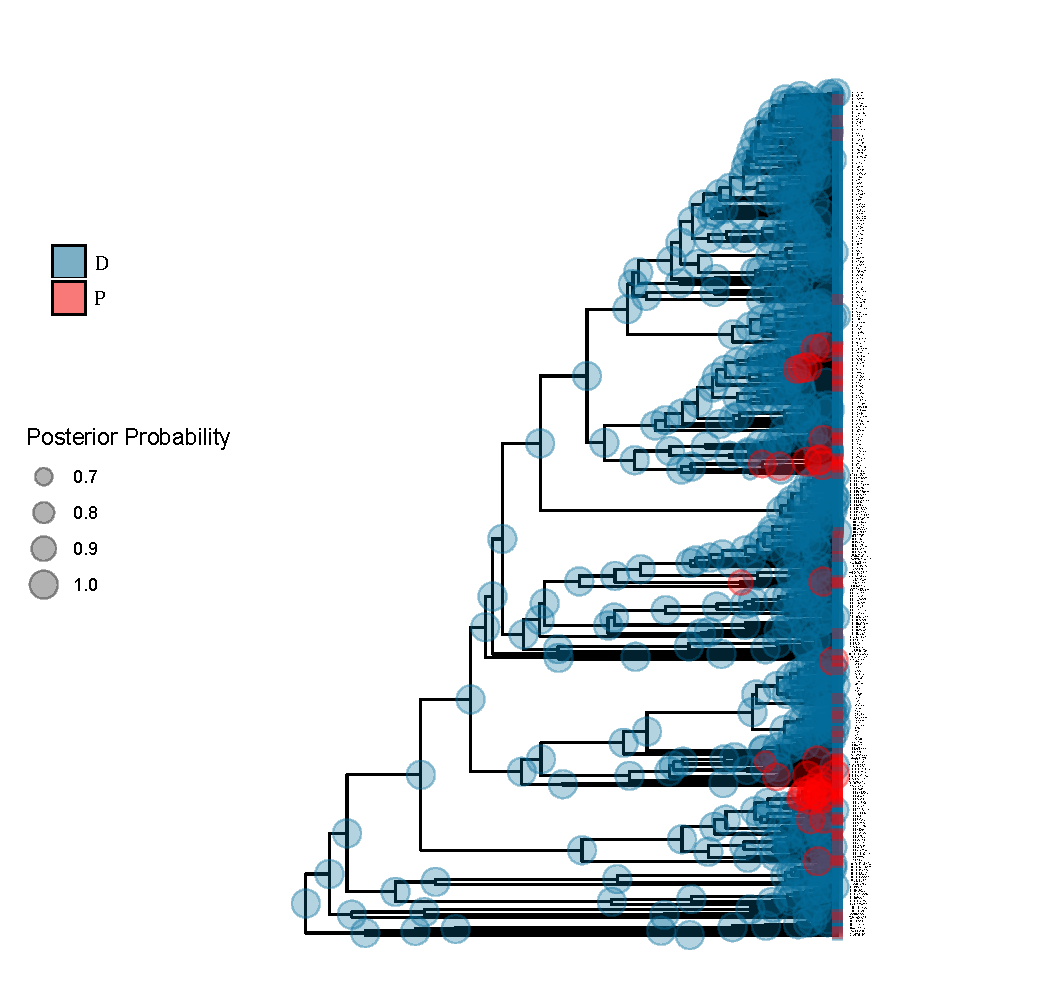
\includegraphics[width=\textwidth]{asrDP.pdf}
\caption{Ancestral state estimation using the maximum a posteriori for each node of theM1. D/P ploidy model} % XXX
\label{suppfigure:DPnodipasr}
\end{suppfigure}

\begin{suppfigure}
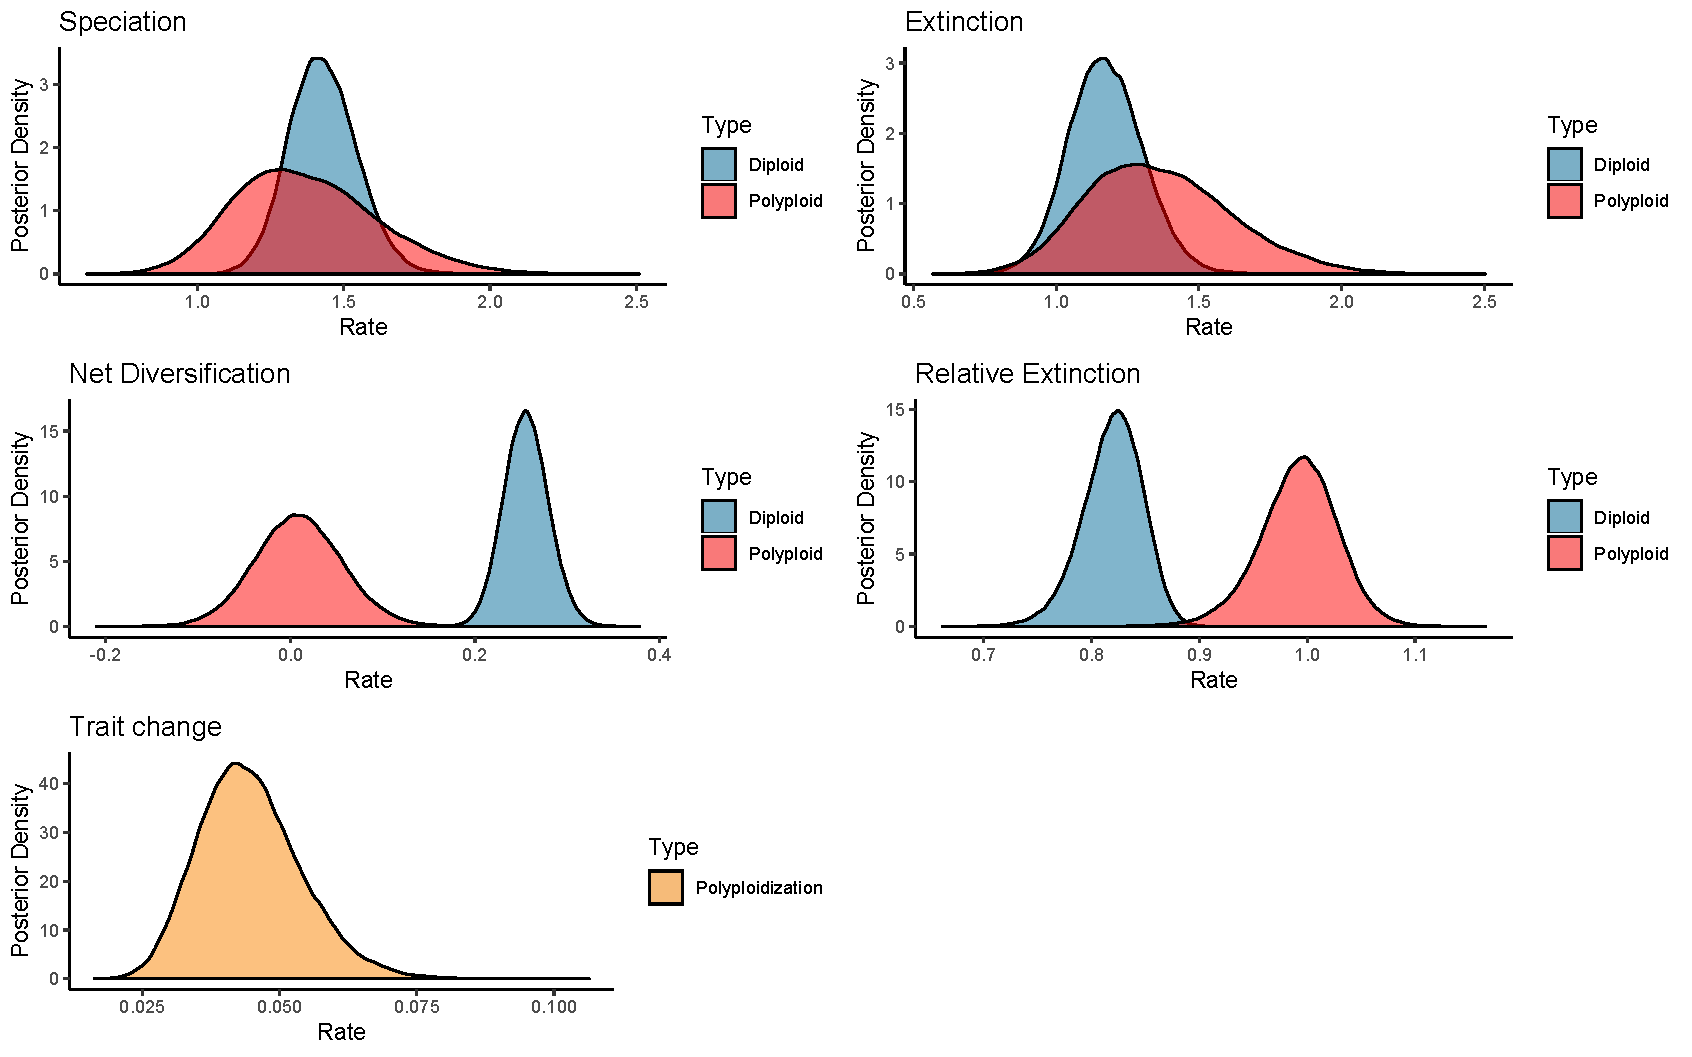
\includegraphics[width=\textwidth]{bisseDPnodipposteriordist.pdf}
\caption{Posterior distribution for each of the parameters in the M1. D/P model} % XXX
\label{suppfigure:DPnodip}
\end{suppfigure}

\begin{suppfigure}
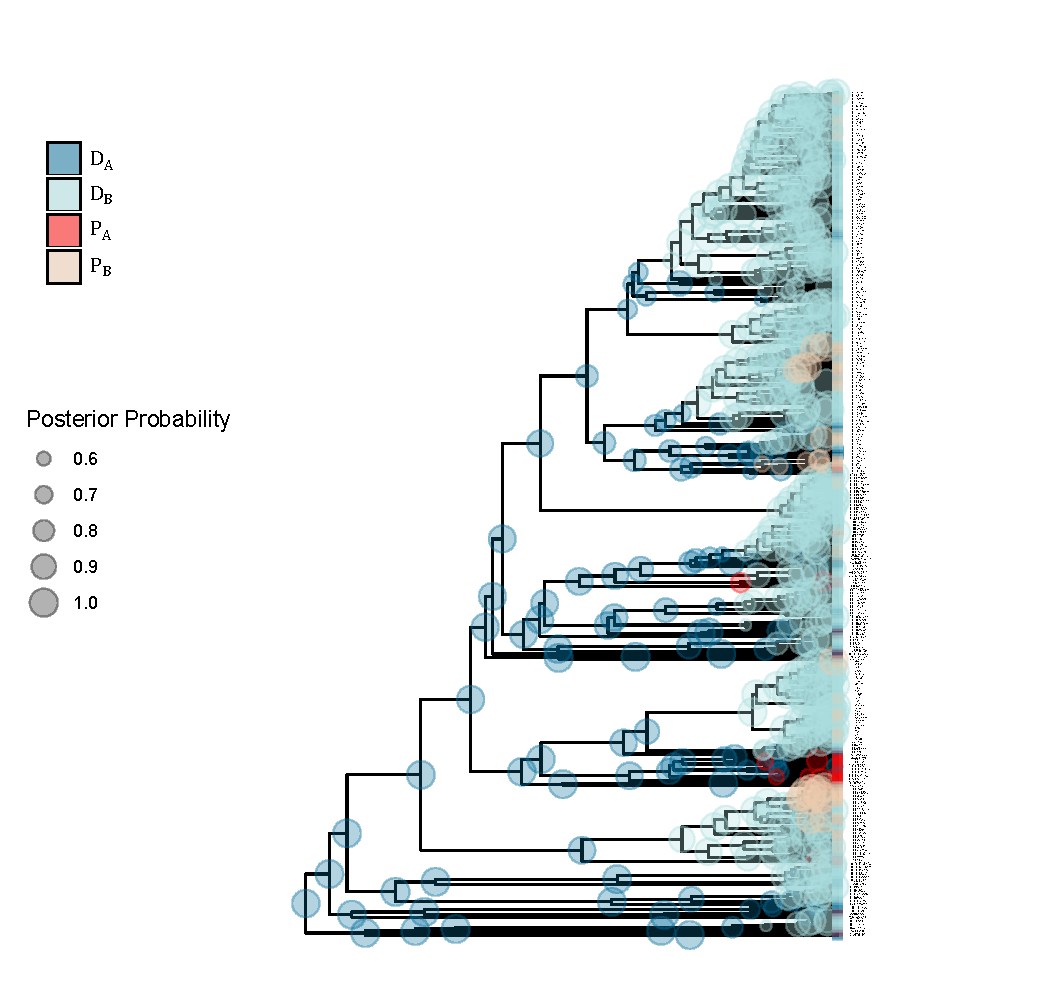
\includegraphics[width=\textwidth]{asrDPAB.pdf}
\caption{Ancestral state estimation using the maximum a posteriori for each node of the M4. D/P+A/B asym model} % XXX
\label{suppfigure:DPnodipABasr}
\end{suppfigure}

\begin{suppfigure}
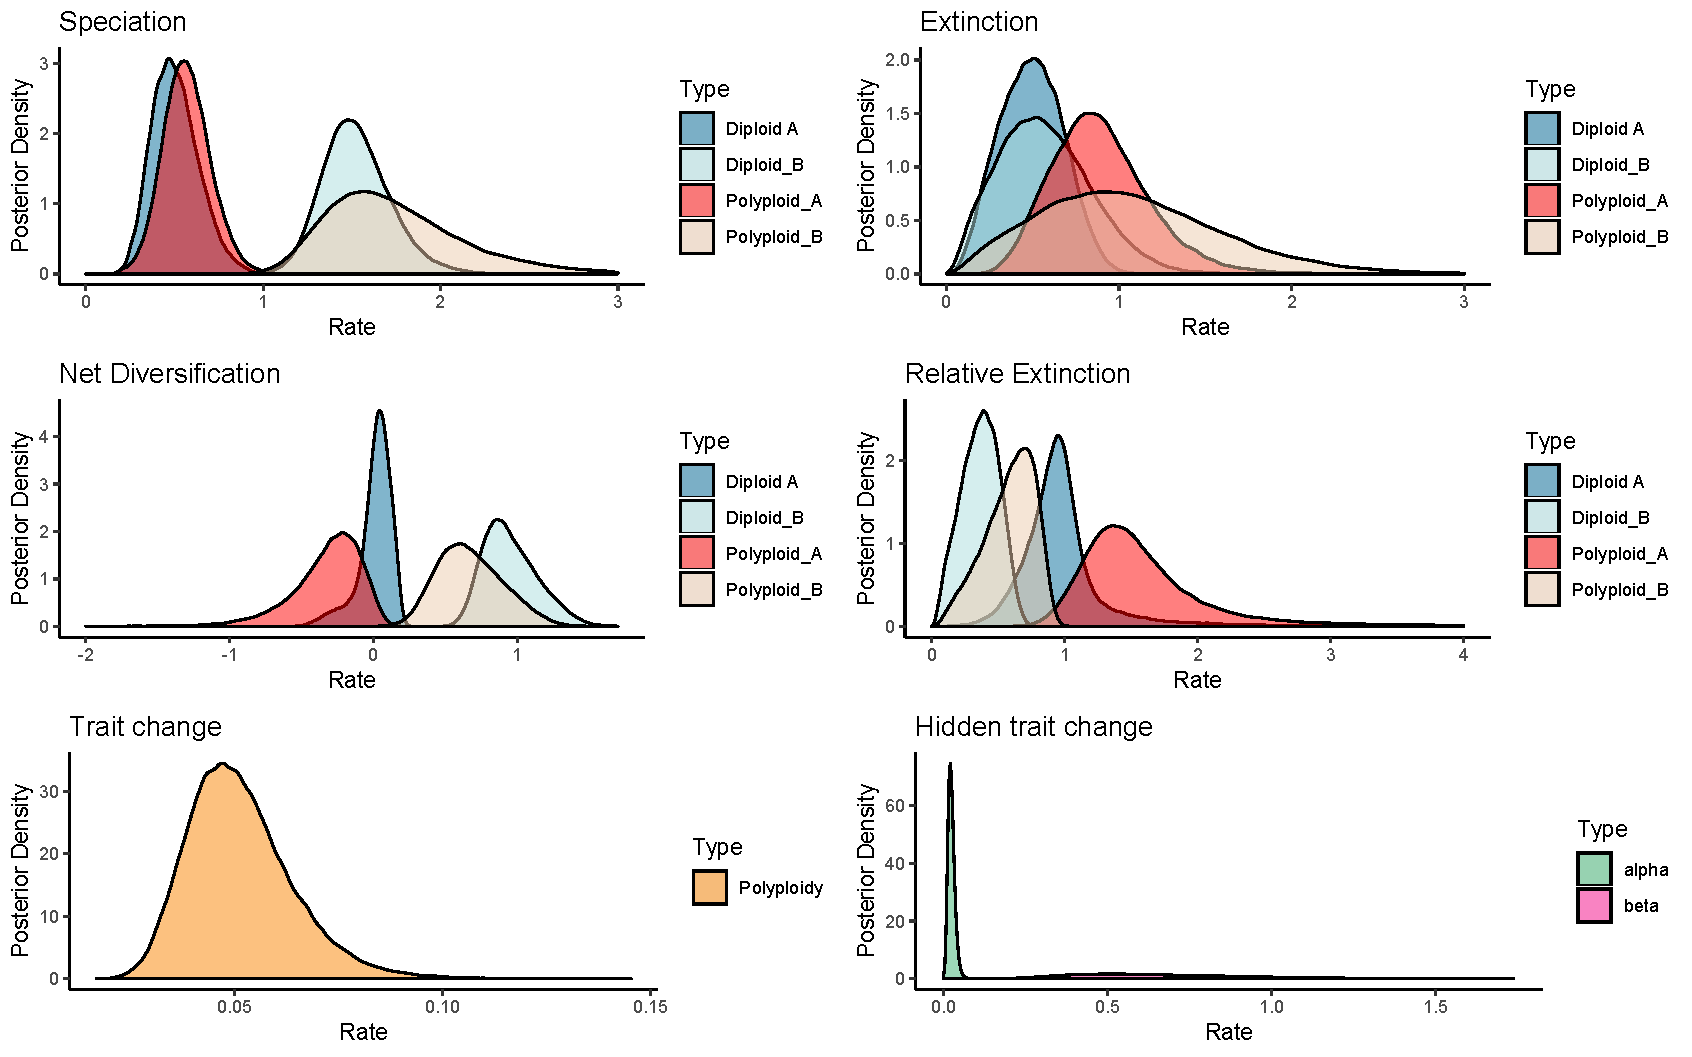
\includegraphics[width=\textwidth]{hisseDPnodipasymposteriordist.pdf}
\caption{Posterior distribution for each of the parameters in the M4. D/P+A/B asym model} % XXX
\label{suppfigure:DPnodipAB}
\end{suppfigure}

\begin{suppfigure}
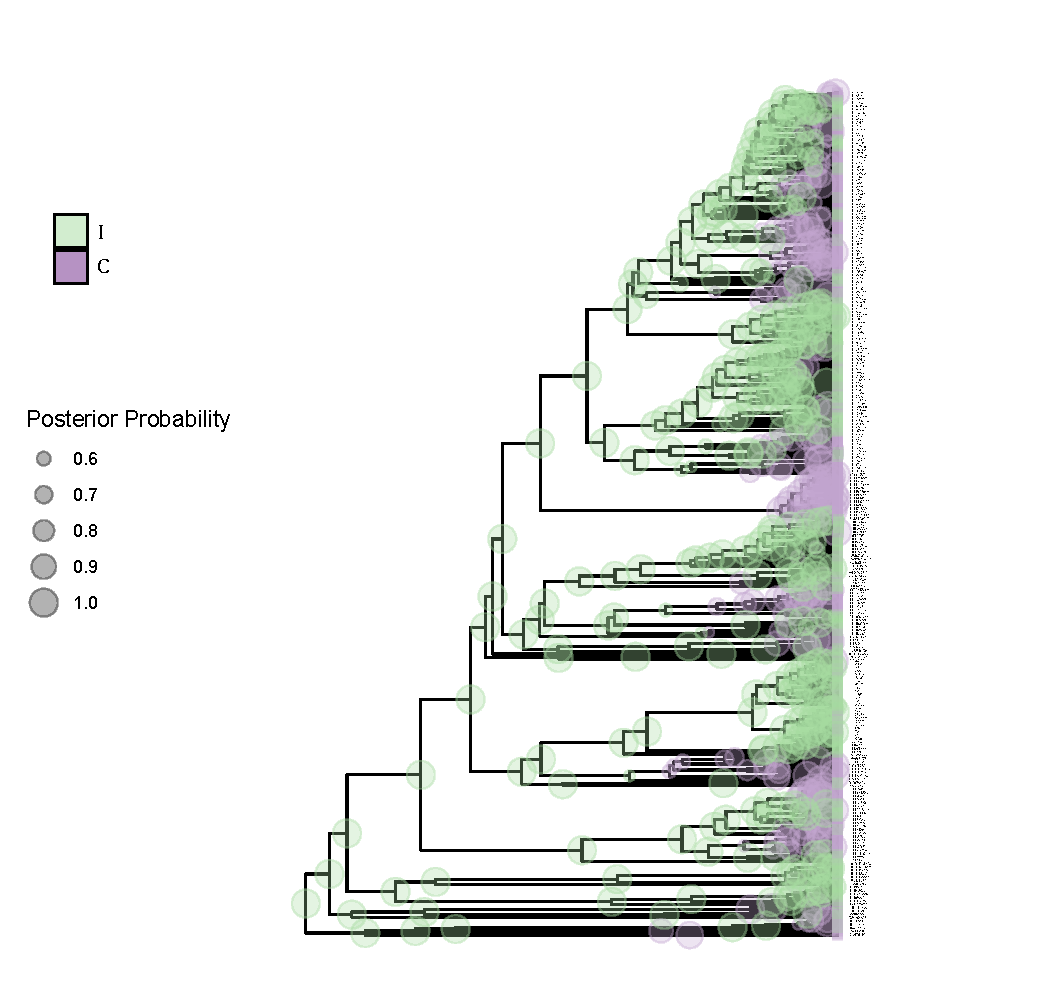
\includegraphics[width=\textwidth]{asrIC.pdf}
\caption{Ancestral state estimation using the maximum a posteriori for each node of the M11.I/C model} % XXX
\label{suppfigure:ICasr}
\end{suppfigure}


\begin{suppfigure}
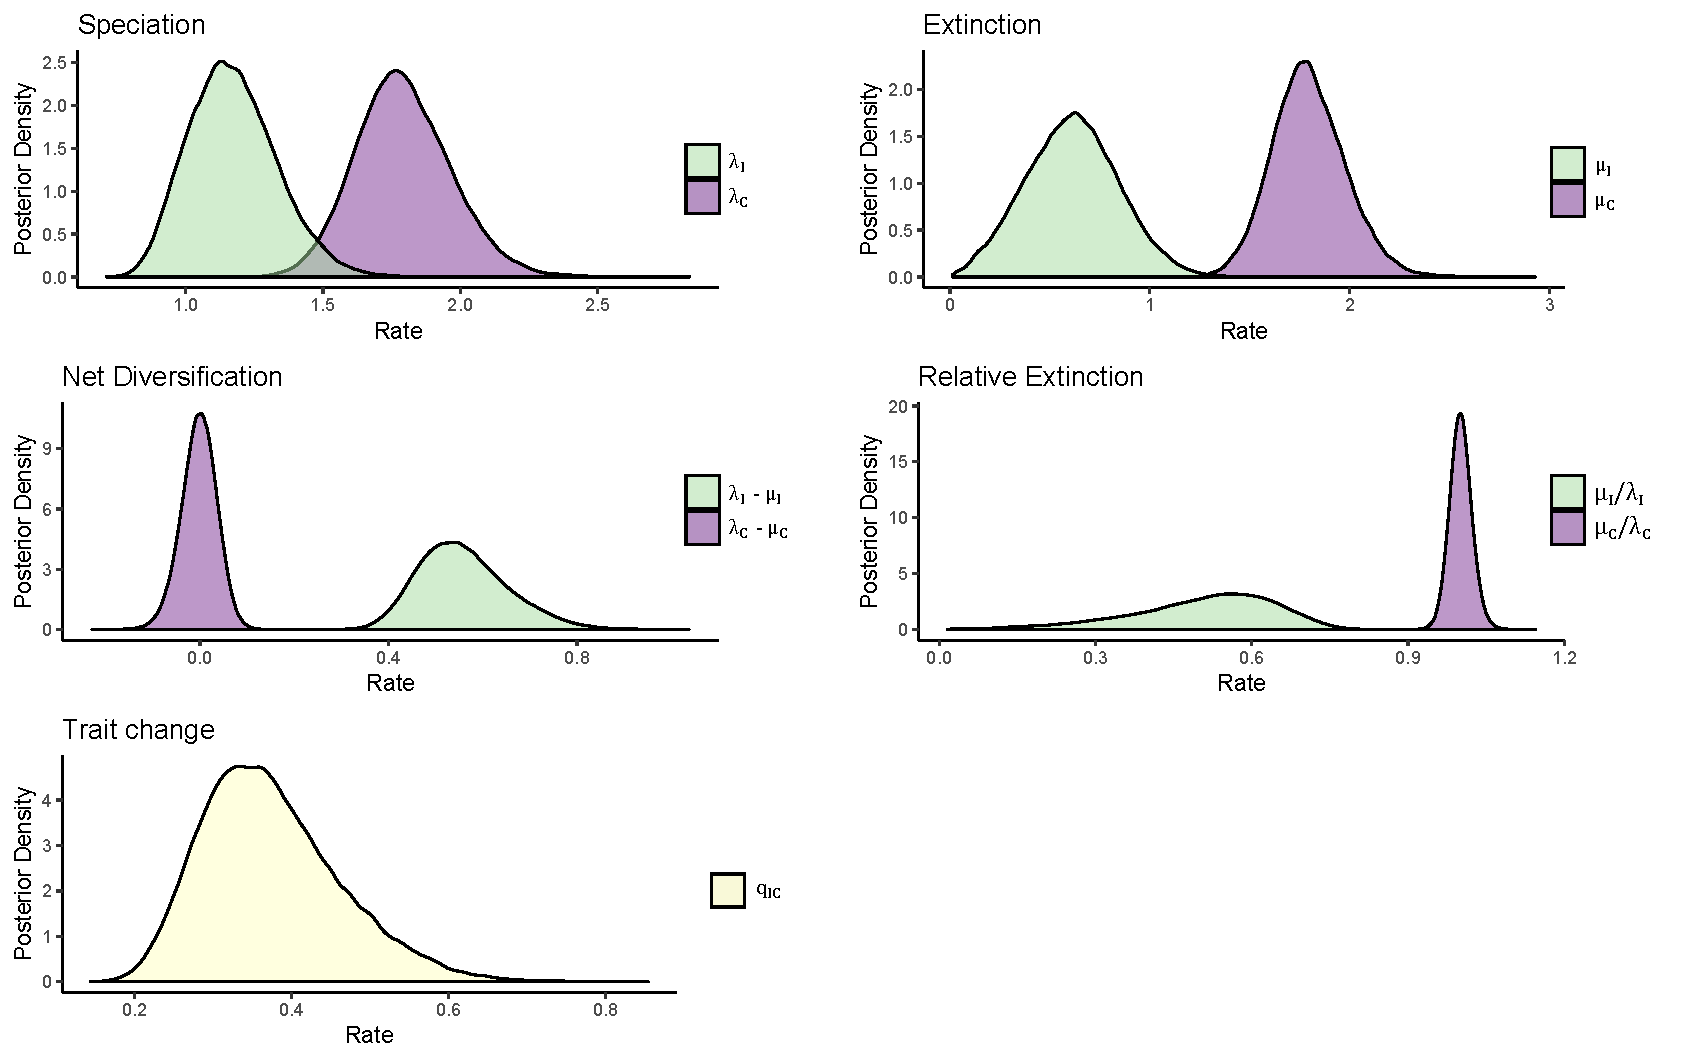
\includegraphics[width=\textwidth]{bisseSIposteriordist.pdf}
\caption{Posterior distribution for each of the parameters in the M11. I/C model} % XXX
\label{suppfigure:IC}
\end{suppfigure}

\begin{suppfigure}
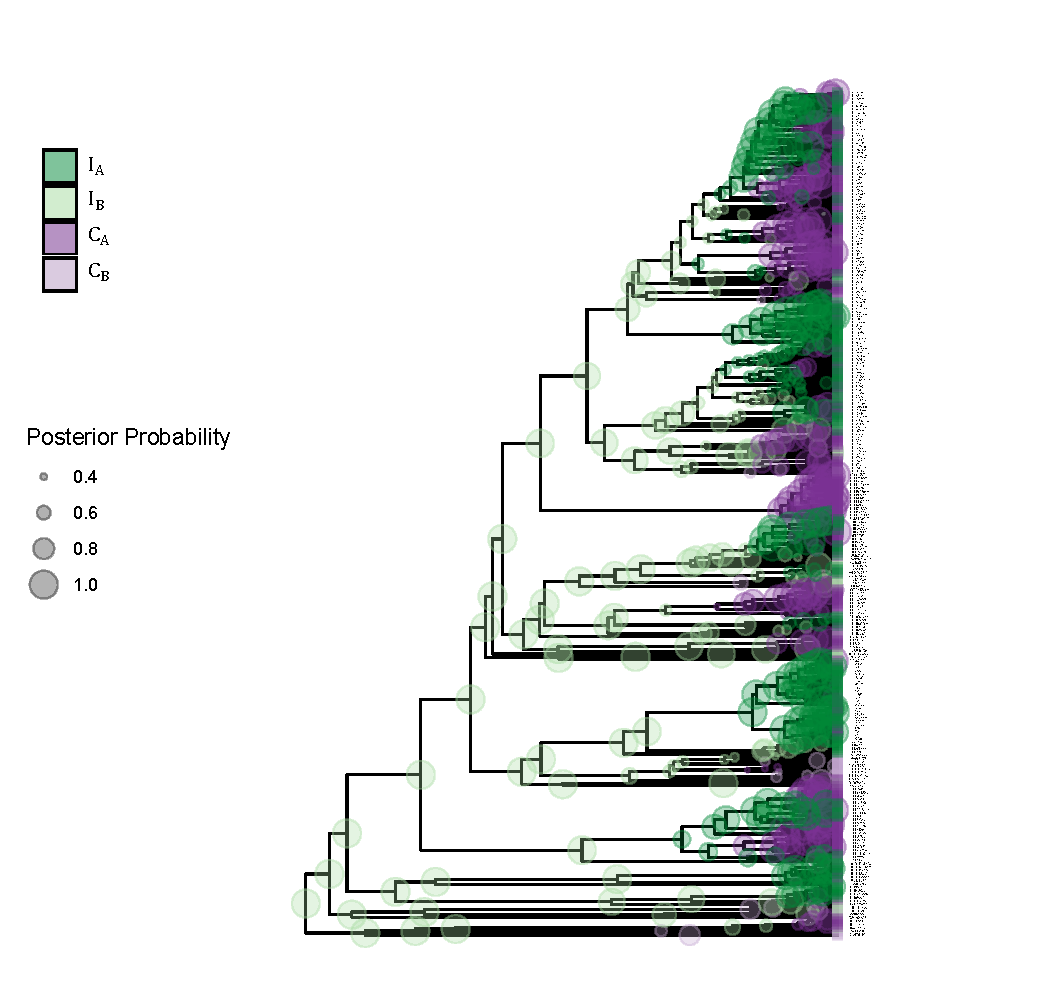
\includegraphics[width=\textwidth]{asrICAB.pdf}
\caption{Ancestral state estimation using the maximum a posteriori for each node of the M14. I/C+A/B asym model} % XXX
\label{suppfigure:ICABasr}
\end{suppfigure}

\begin{suppfigure}
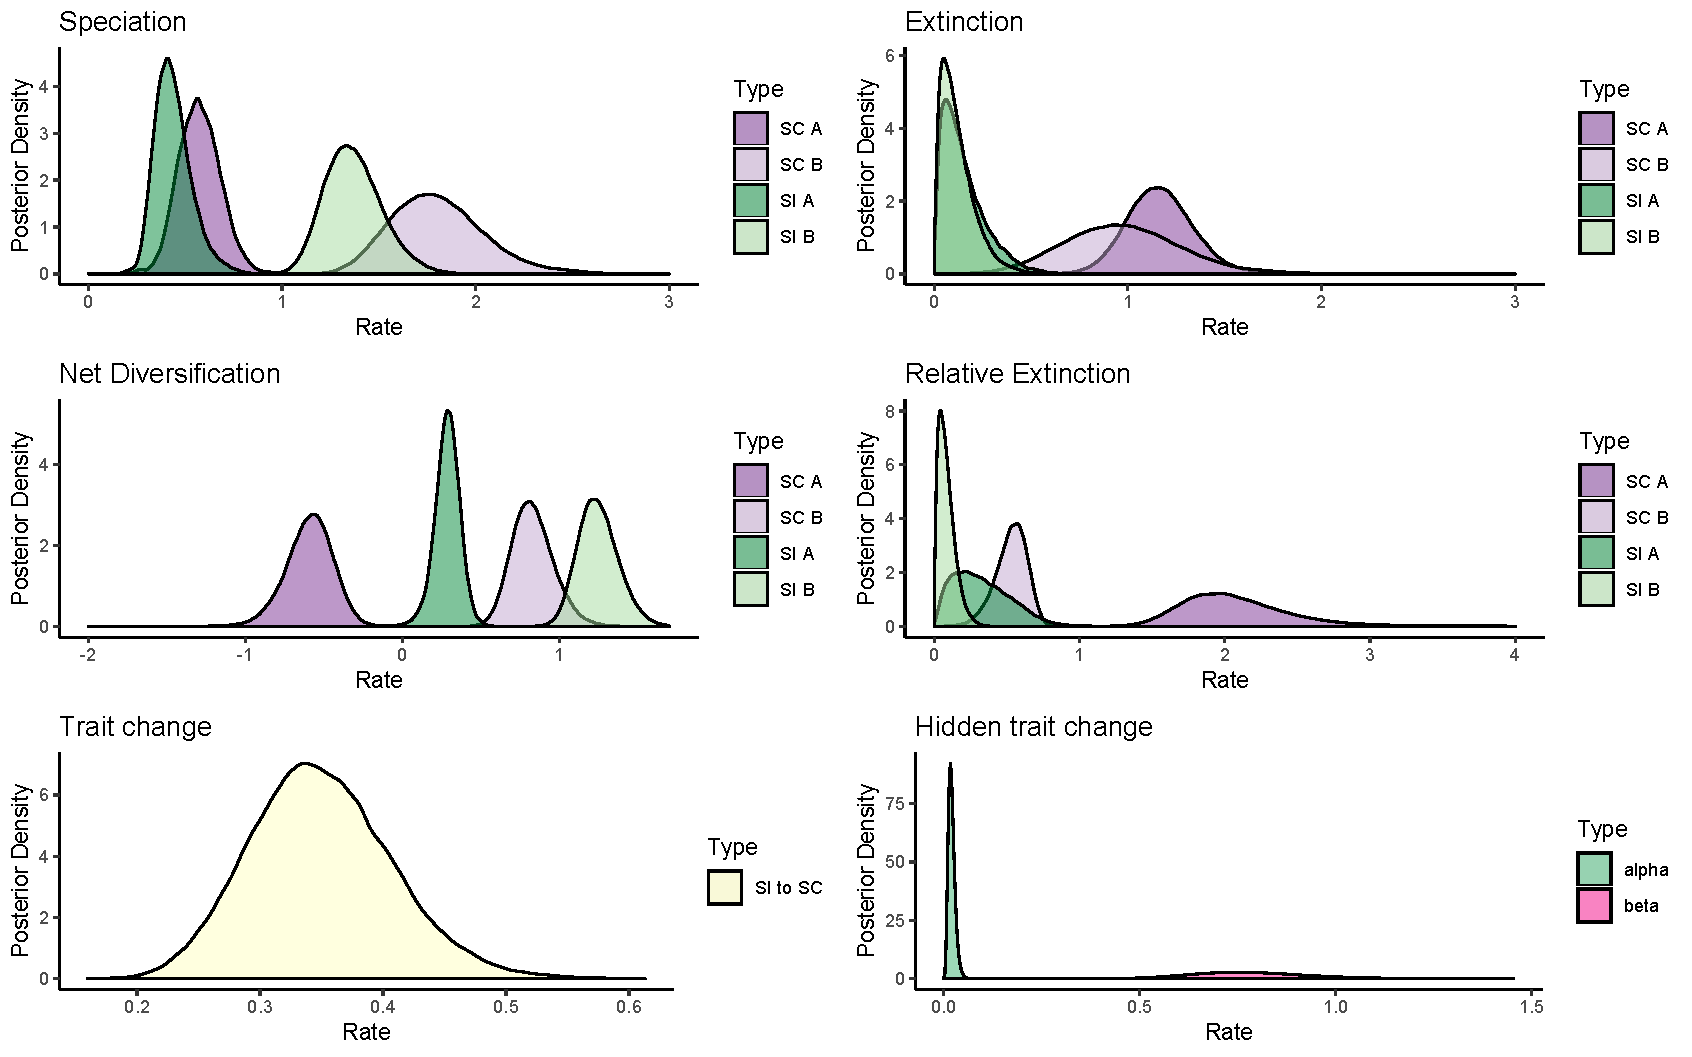
\includegraphics[width=\textwidth]{hisseSIasymposteriordist.pdf}
\caption{Posterior distribution for each of the parameters in the M14. I/C+A/B asym model} % XXX
\label{suppfigure:ICAB}
\end{suppfigure}

\begin{suppfigure}
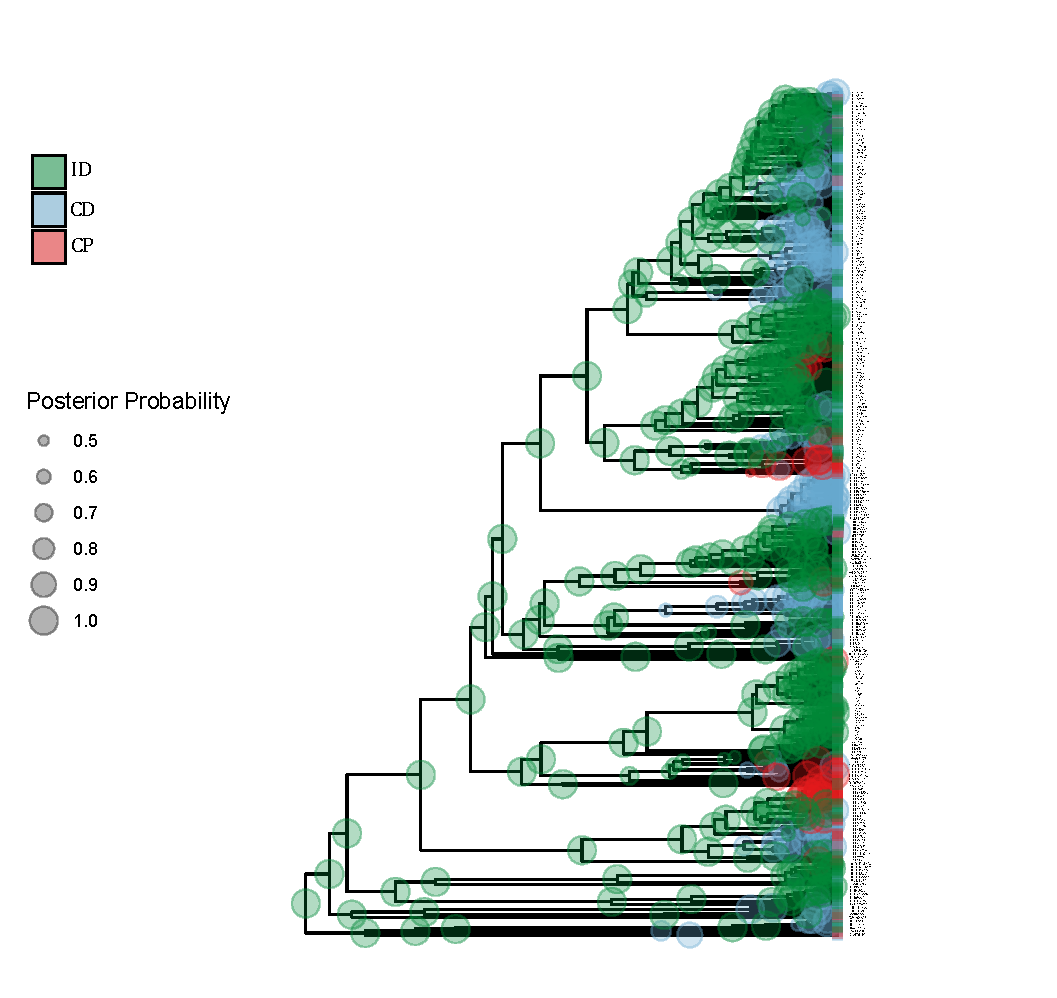
\includegraphics[width=\textwidth]{asrIDCDCP.pdf}
\caption{Ancestral state estimation using the maximum a posteriori for each node of the  M16. ID/CD/CP model} % XXX
\label{suppfigure:IDCDCPnodipasr}
\end{suppfigure}


\begin{suppfigure}
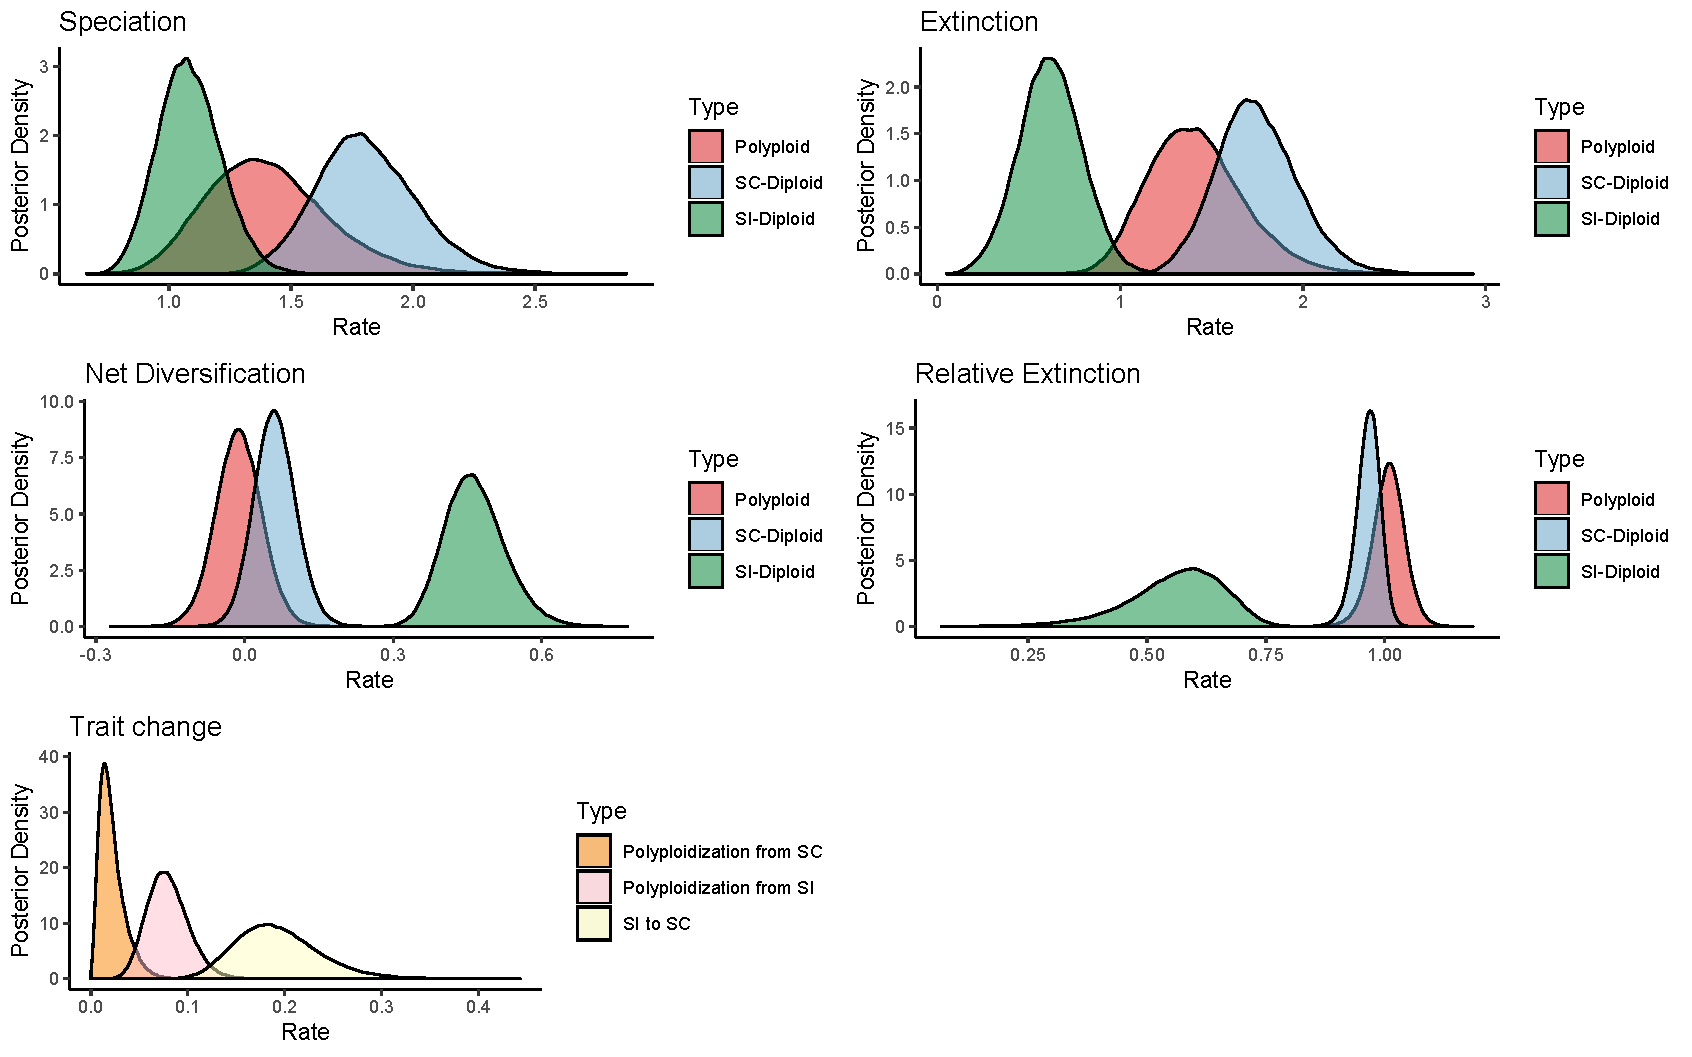
\includegraphics[width=\textwidth]{musseDPSInodipposteriordist.pdf}
\caption{Posterior distribution for each of the parameters in the  M16. ID/CD/CP model} % XXX
\label{suppfigure:IDCDCPnodip}
\end{suppfigure}

\begin{suppfigure}
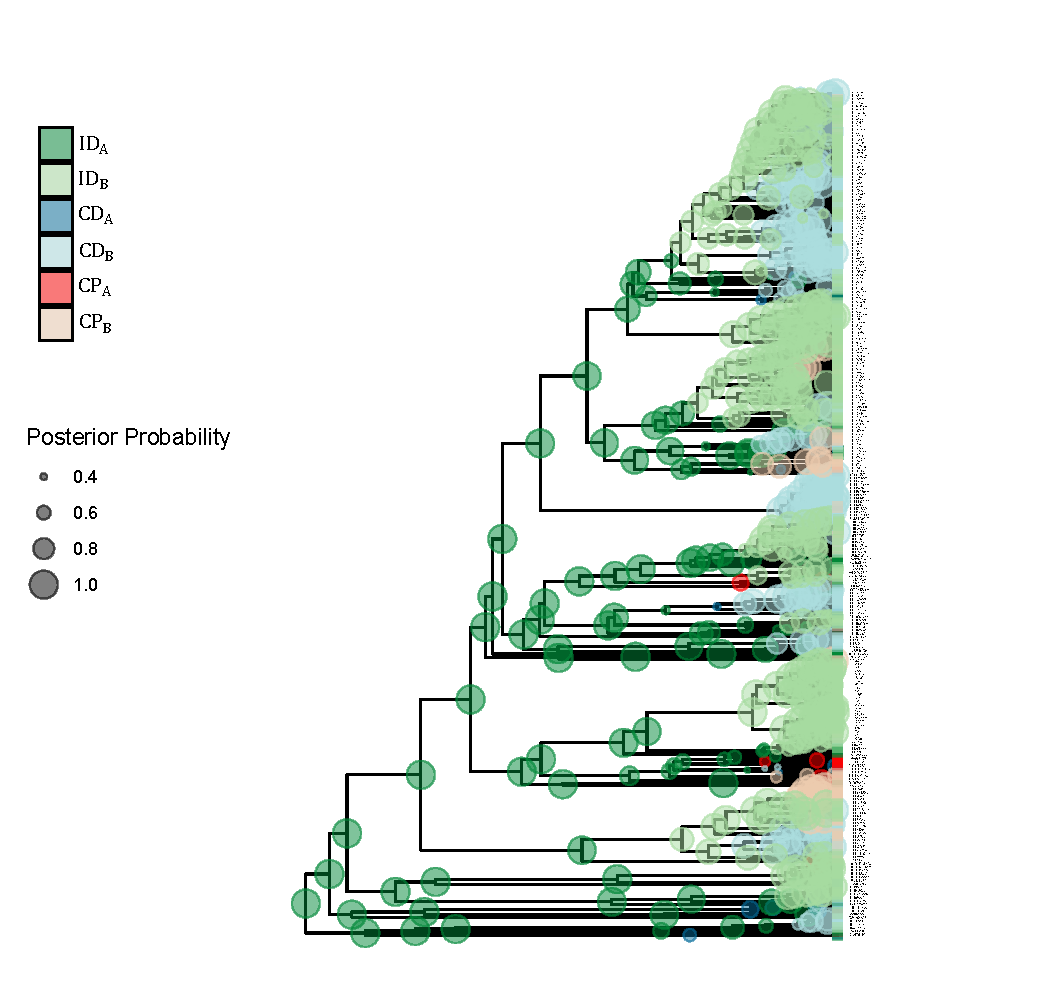
\includegraphics[width=\textwidth]{asrIDCDCPAB.pdf}
\caption{Ancestral state estimation using the maximum a posteriori for each node of the  M19. ID/CD/CP+A/B asym model} % XXX
\label{suppfigure:IDCDCPnodipABasr}
\end{suppfigure}


\begin{suppfigure}
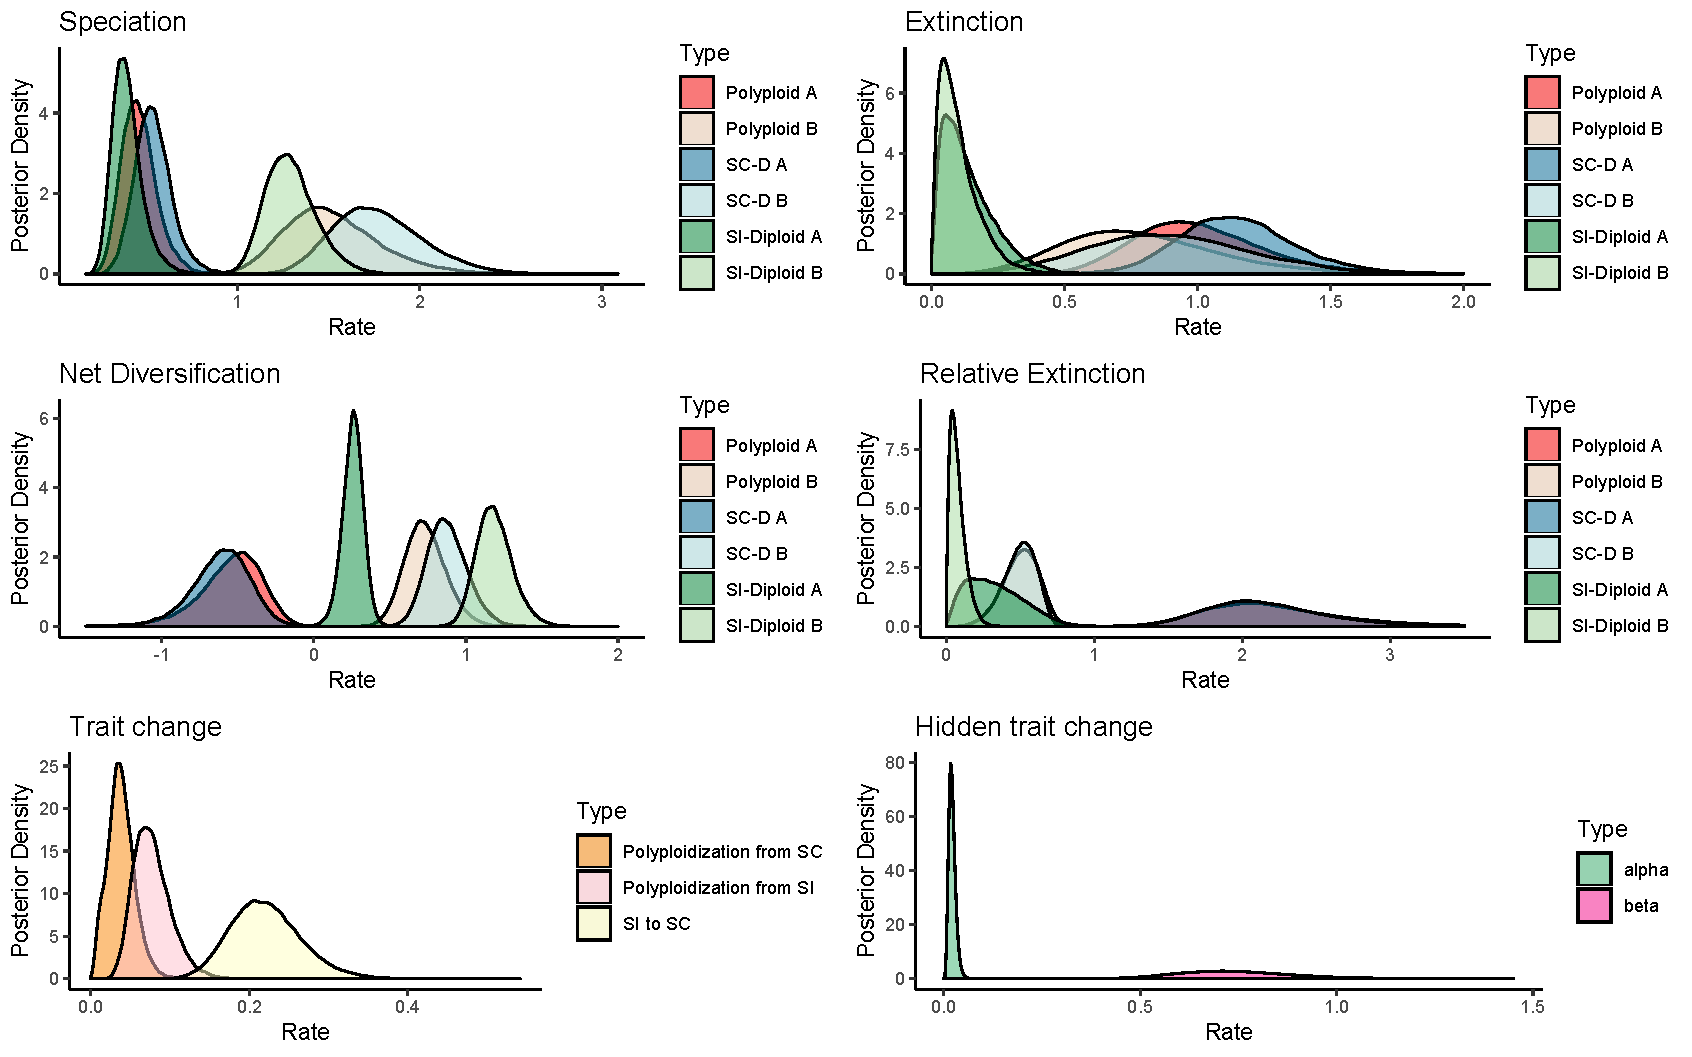
\includegraphics[width=\textwidth]{muhissenodipasymposteriordist.pdf}
\caption{Posterior distribution for each of the parameters in the M19. ID/CD/CP+A/B asym model} % XXX
\label{suppfigure:IDCDCPnodipAB}
\end{suppfigure}
